\documentclass[dvipdfmx,twocolumn]{jsarticle}
\usepackage{graphicx}
\usepackage{latexsym}
\usepackage{amsmath}
\usepackage{url}
\begin{document}
    \title{SSL/TLSを回避する中間者攻撃の新たな提案とその脅威\\~実装による評価と考察~}
    \author{木村 圭一朗\thanks{神戸大学工学部電気電子工学科\\Department of Electrical and Electronic Engineering, Faculty of Engineering, Kobe University} \and 森井昌克\thanks{神戸大学大学院工学研究科\\Graduate School of Engineering, Kobe University} \and 白石善明\thanks{神戸大学大学院工学研究科\\Graduate School of Engineering, Kobe University}}
    \date{}
    \begin{abstract}
        昨今のインターネットの著しい普及により,屋外で利用できるネットワークの需要が拡大している.\
        その需要に応える通信インフラとして公衆無線LANがあり,公共のあらゆる場でその整備が進んでいる.\
        しかし,セキュリティ面での懸念は依然として残っている.\
        利用した公衆無線LANが通信の傍受を目的とした悪性のものである可能性は,その懸念の一例である.
        屋外で手軽にインターネットを利用できる反面,ユーザーたちはその公衆無線LANの提供元を確認することはほとんどないだろう.\
        近年は通信内容が暗号化されたHTTPS通信が主流になり,中間者攻撃に対する対策も行われているが,公衆無線LANを利用した通信の場合はそれが容易に可能になる場合がある.\
        本研究では,公衆無線LANにおけるCaptive Portalを起点とした通信の傍受・窃取を行う手法について提案する.また,前述の手法の実装を行い,加えてその評価も行った.\\
    \end{abstract}
    \maketitle
    \section{導入と背景}
        スマートフォンの普及に伴う屋外の快適なネットワーク環境の需要が高まっており,その具体的なインフラとして,公衆無線LANが挙げられる.\
        現在では,公衆無線LANは日常の様々な側面に溶け込んでおり,その一例として,新幹線や飛行機,カフェや宿泊施設など,日常生活に欠かせない施設が挙げられる.\
        総務省は,災害時の情報収集や通信手段として,また観光情報の収集や教育現場での活用による利便性の向上を目指し,平成30年までに全国約3万箇所に公衆無線LANを設置する案をまとめた\cite{SoumuWiFi}.\\
         このように,公衆無線LANの普及が加速的に行われている中,そのセキュリティ対策も課題となっている.\
        特に,公衆無線LANには,大衆利用を想定した特性上の多くの脅威が潜んでおり,IPA(独立行政法人情報処理推進機構)による「公衆無線LAN利用に係る脅威と対策~公衆無線LANを安全に利用するために~」の資料\cite{IPA}には,主に以下の4つの脅威が示されている.\
        \begin{enumerate}
            \item 盗聴
            \item なりすまし
            \item 悪意のAP(AP:アクセスポイント)
            \item 不正目的でのインフラの利用
        \end{enumerate}
         「盗聴」とは,無線通信の傍受・窃用を意味するが,公衆無線LANの様なアクセスに必要な情報が不特定多数の利用者に共有された状態の場合,たとえ暗号化された通信でも,その復号に必要な情報を得る事が可能なため,通信内容の盗聴の脅威が十分にある.\
        「なりすまし」とは,MACアドレスの偽造により,本来接続できない端末に対して第三者が接続・操作することを指す.\
        この行為は,MACアドレスを登録した端末とのみ無線通信を行うMACアドレスフィルタリングという機能を利用することで可能になる.\
        「悪意のAP」とは,第三者が悪意ある目的で設置されたアクセスポイントを指す.\
        この場合,利用者が正規のアクセスポイントと誤認して悪意あるアクセスポイントを利用した場合,個人情報などの機密性・重要性の高い情報が抜き取られるという脅威がある.\
        「不正目的でのインフラの利用」とは,例えばユーザーの認証を行わないような公衆無線LANの場合,利用者の特定が困難さを逆手に取ったサービスの不正利用を行うインフラと化してしまう.\
        このように,公衆無線LANには様々な脅威が潜んでおり,その対策は現在も大きな課題となっている.\\
         本研究では,上記の4つの脅威の中の「悪意あるAP」に着目し,「悪意あるAP」を起点とした中間者攻撃の手法ついて議論している.\
        「悪意あるAP」には,そもそも通信内容の傍受・窃取や機密性の高い情報の盗聴を目的として設置されたものが多いため,その攻撃起点は様々であり,アクセスポイントの利用者が,一般的な利用者,つまりインターネットや通信・セキュリティに関する専門的知識を有さない者を想定した場合,利用者はその脅威を認識することは非常に困難である.\
        Captive Portalはその攻撃起点として利用されることが多く,その攻撃手法に対する対策は,既に多くの研究で十分に議論されている.\
        例えば,LUNODZO J. MWINUKAらは,正規APになりすましてMITM攻撃を行うような悪意あるAPの検出を行うAndroidアプリケーションの開発を行った\cite{FakeAP}.\
        その中で,Captive Portalを起点として認証情報の窃取を行うような悪意あるAPに対し,ランダムな認証情報の入力を行うことで対象のAPの真正性を確認する手法を提案している.\
        また,Vineeta Jainaらは,ビーコンフレームからフィンガープリントを生成し,その情報とSSIDや信号強度との比較を行うことでワイアレスEvil Twinsへの接続を未然に防止するET Guardというアプリケーションを開発した\cite{ETGuard}.\
        そこで想定されている攻撃シナリオとして,ユーザーが悪意あるインテントが組み込まれたアプリケーションをインストールしているという前提のもと,Evil Twinsが提供するCaptive Portalを起点として,その悪性あるインテントを起動させてポート開放などの危険性を生み出す手法が想定されている.\
        ET GuardはそれらのAPに接続する前に検出を行うことでインテントの起動を未然に防いでいる.\
        しかし,これらの想定された攻撃手法は,偽APが提供するCaptive Portalの認証画面を起点としたもので,認証後に遷移させる画面を起点とした攻撃は議論されていない.\\
         中間者攻撃とその対策についても,これまでの研究で十分に検討されている.\
        SSL/TLS通信に対する中間者攻撃として,2009年のBlack HatでMoxie Marlinspike氏によって提案されたSSL Strip攻撃がある\cite{SslStrip}.\
        これは,クライアントと攻撃者間の通信をHTTPS通信からHTTP通信へ置換することで,クライアントの機密情報を傍受・窃取する手法である.\
        この手法に対しては,Webサイトがブラウザに対してHTTPの代わりにHTTPSを用いて通信を行うように強制するHSTS(HTTP Strict-Transport-Security)を用いることでその実行を防ぐことが可能となった.\
        Takashi Setozakiの研究\cite{HSTS}によれば,クライアントがアクセスしようとしているドメインがブラウザのHSTSリストに存在しない前提のもと,サーバから送られてきたHTMLファイル内の"https://"から始まるリンクに対して,そのドメイン名をHTTPS接続する直前にHTTP接続していたドメインにすり替えることでHSTSを回避するSSL Strip攻撃の手法を提案した.\
        しかし,前提条件にもあるように,対象のドメインがHSTSリストに存在した場合はこの手法によるSSL Strip攻撃は困難と考えられる.\
        また,東海大学の菊池研究チームらの研究\cite{FakeSslAndDnsServer}では,偽造DNSサーバを構築することで通信を攻撃サーバを経由させるようにし,且つ任意のサーバに対して証明書を自動的に作成するプログラムを構築することで,動的にSSL中間者攻撃を行う手法が提案されている.\
        サーバの偽造証明書は,Open SSLを用いて正規サイトのサーバ証明書を偽装した自己署名証明書を作成することで実現させている.\
        しかし,結果として生成された証明書は本来の証明書を完全に偽造することは不可能とされており,ブラウザによる証明書検証の際の警告出現の可能性は拭えているとは言えない.\\
         本研究では,このCaptive Portalの仕組みを起点とし,攻撃者がクライアントとサーバ間の通信に割り込む形をつくることで,通信がSSL/TLS通信でも,且つクライアントのブラウザに警告を出さずに通信内容及び機密情報の傍受・窃取を行う手法を考え,その攻撃に成功した.\
        既存の研究では,偽のCaptive Portalを利用した認証情報の窃取に対する対策は講じられているが,本研究ではクライアントの認証情報の窃取は主な目的としてない.\
        Captive Portalを用いる主な目的は,攻撃者が通信の中継形態をつくる為に,認証後に遷移させる偽のWebサイトに飛ばす事である.\
        具体的には,認証後に偽の検索エンジンに誘導させる事で通信の中継機会をつくり,ターゲットをメジャーな通販サイトに絞って,その個人情報の傍受・窃取を成功させた.\
        加えて,その傍受・窃取を行うシステムに対しての可能性と課題の評価を行った.\
    \section{前提条件}
        今回,MITM攻撃を仕掛けるにあたり以下の前提条件を設けた.\\
        \\
        利用者は
        \begin{itemize}
            \item 偽SSIDを有する無線LANアクセスポイント(以下,AP)を使用する.
            \item HTTPS通信で任意のサイトを閲覧する.
            \item 通信先を確認しない.
        \end{itemize}
         まず,偽SSIDを有するAPを利用するという前提条件について説明する.\
        攻撃者が利用者の通信の内容を盗み見る為には,利用者を攻撃者が用意したAPへ接続させる必要がある.\
        しかし,通常の公衆のAPのSSIDは,それを提供している施設や会社の名前に関連したものが多く,利用者も提供元の名前に関連したSSIDを有するAPに接続を試みる.\
        従って,攻撃者が用意したAPのSSIDも,利用者が施設や会社が提供したWiFiであると誤認させる様なSSIDを用いるという前提が必要である.\\
         次に,利用者はHTTPS通信でサイトを利用するという条件について,これは現在のWebサイト,特に個人情報やクレジットカード番号など機密性・重要性の極めて高い情報を扱うようなWebサイトは,常時HTTPS通信を用いている点にある.\
        特に,中間者攻撃への対抗策としてHSTP(HTTP Strict Transport Security)という,サーバーがブラウザに対してHTTPS通信を強制する様な仕組みが実装されているものもある.\
        従って,通信内容に対して暗号化が施されていないHTTP通信を前提としての検証は現実的でない為,HTTPS通信を想定する必要がある.\\
         最後に,通信先を確認しないという前提についてであるが,これは一般的な利用者の想定を意味する.\
        通常,ネットワークについての知識が深い利用者や,セキュリティリテラシーの高い利用者は,閲覧しているサイトのドメインの確認などを通して正規サーバとの通信を確認するが,一般的な利用者はそのような確認は行わない.\
        本研究は公衆無線LANを用いる一般的な利用者を想定している為,通信先の確認は想定しない.\\
    \section{中間者攻撃ツールの開発}
        \subsection{検証対象}
            中間者攻撃が可能か否かの検証にあたり,昨今急激な普及が見られるインターネット通販サイトを対象とした.その中でも国内ECモールの売上ランキング上位2つを占める「楽天」と「Amazon」を対象とした.\
            また,これ以降は,攻撃者が用意した悪意あるAPを「悪性AP」,通信の仲介に用いる攻撃者サーバを「悪性サーバ」をして説明する.
        \subsection{検証フロー}
            主な検証フローは次の通り.各フェーズの具体的な説明は次のサブセクションに記述している.
            \begin{enumerate}
                \item CaptivePortalを検知させて,予め攻撃者が用意しておいたCaptive Portalサイトに誘導し,認証を行わせる.
                \item 認証後,偽の検索エンジンの画面へ遷移させ,被害者が検索したワードを悪性サーバで取得する.
                \item 攻撃者は取得したワードをバックエンドで検索し,その検索結果を取得する.
                \item 取得したHTMLファイル内にあるハイパーリンクを書き換え,そのコピーを被害者に提示する.
                \item 以後,クリックしたURLを悪性サーバで取得する.
                \item 攻撃者は取得したURLを利用して正規サーバにアクセスする.
                \item 正規サーバから返却されたHTMLファイル内のハイパーリンクを書き換え,被害者に提示する.
            \end{enumerate}
        \subsection{実装}
            システムはGolangで実装した.\
            付録に該当のGitHubリポジトリのリンクを載せている.\
            また,APは"GL.iNet GL-AR300M(shadow)無線LAN vpnトラベルルーター Openwrtインストール 中継器ブリッジ 11n/g/b 高性能300Mbps 128MB Nand フラッシュ OpenVPN/WireGuardクライアント/サーバー 日本語界面"を使用し,認証後に実装したシステムに飛ばすように設定した.\
            ここでは,各検証フローについて具体的な実装内容を示す.\
            \subsubsection{検証フロー1,2について}
                図\ref{flow-no12}に,具体的な挙動を示す.\
                まず,被害者は疑うことなく悪性APへの接続を試みるとする,\
                使用しているAPはCaptive Portalを実装している為,接続要求をした被害者デバイスに対して認証を行うように命じる.\
                認証が終了すると,攻撃者が用意した悪性サーバに飛ばす.\
                今回は,悪性サーバは偽の検索エンジンを装い,被害者はそれを疑うことなく用いるとする.\
                \begin{figure*}[t]
                    \centering
                    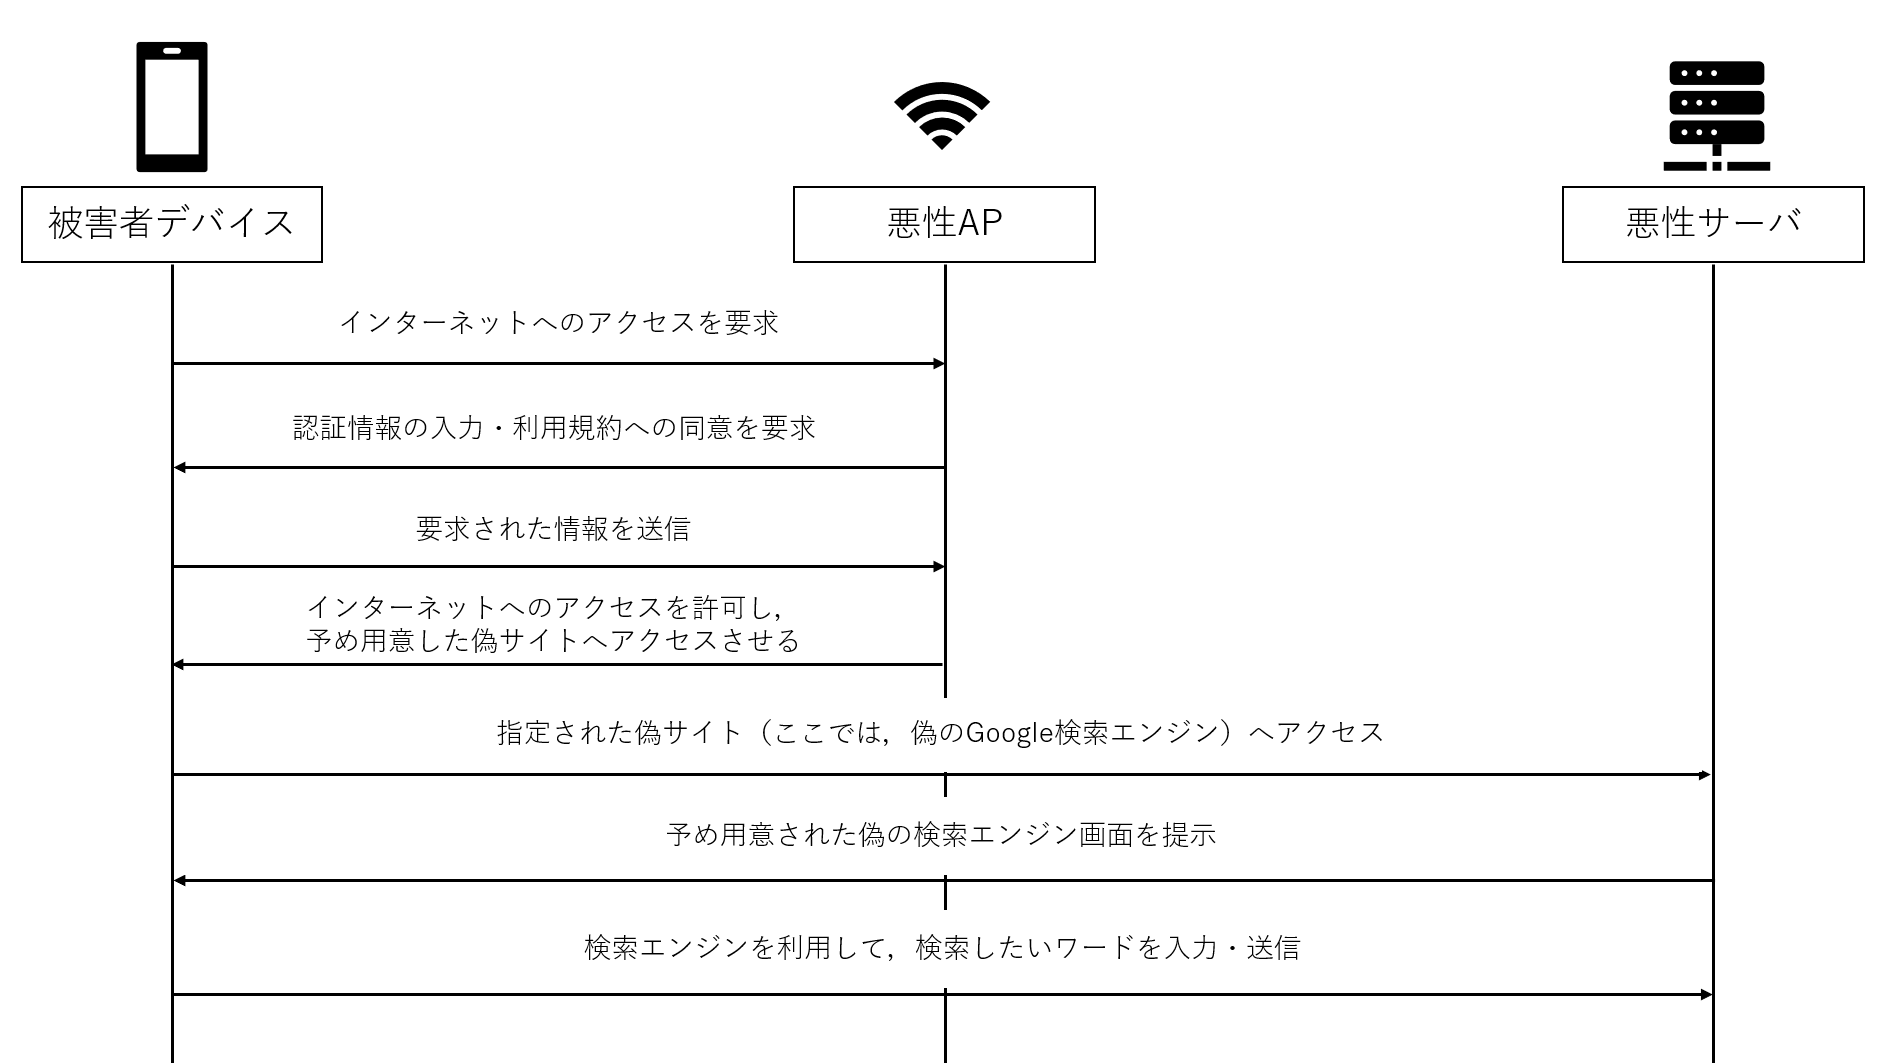
\includegraphics[width=12cm]{img/vc-vf-1-2.png}
                    \caption{偽のAPとCaptive Portalの仕組みを仕様して,偽の検索エンジンに飛ばすまでの挙動}
                    \label{flow-no12}
                    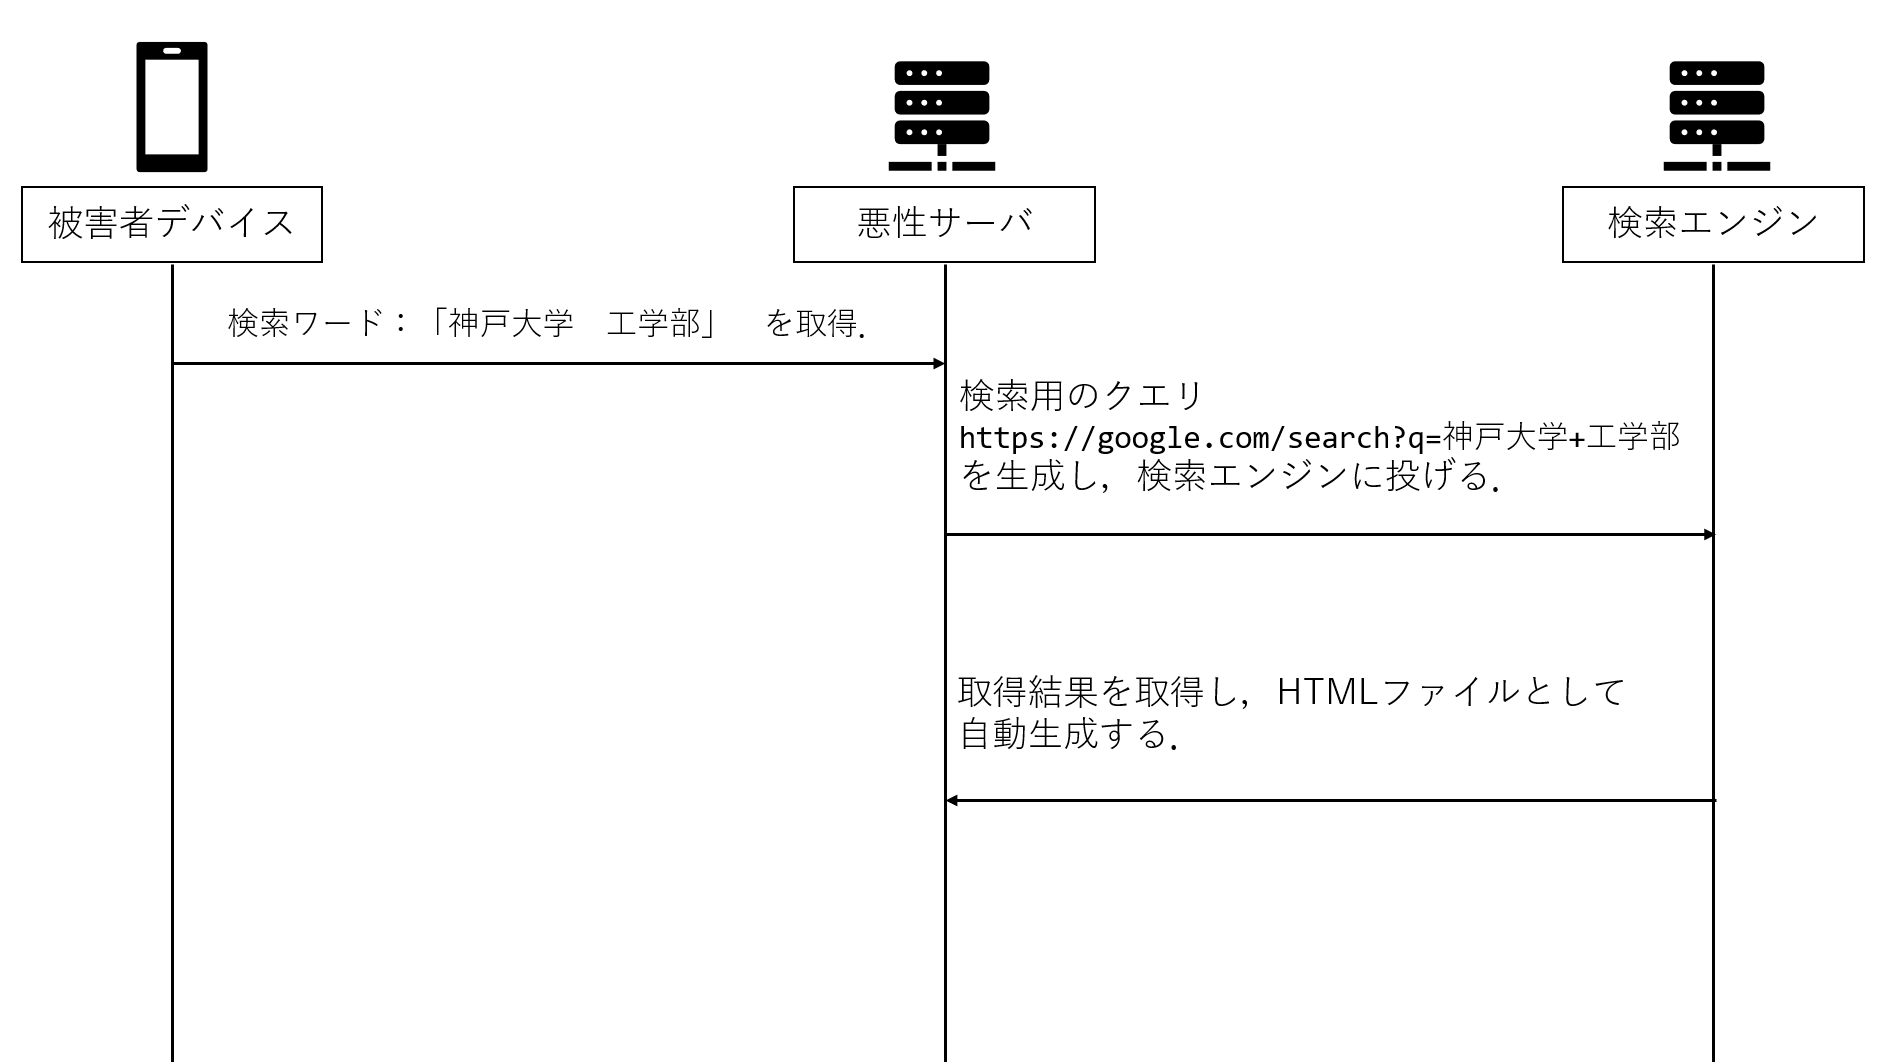
\includegraphics[width=12cm]{img/vc-vf-3.png}
                    \caption{検索ワードを取得してから,検索結果を取得するまでの流れ}
                    \label{flow-no3} 
                \end{figure*}
            \subsubsection{検証フロー3について}
                ここでは,最も利用されているGoogleの検索エンジンを用いた.\
                Googleでの検索結果を取得する為には,検索クエリを作成する必要がある.\
                基本的に任意のクエリ(query)に対して https://google.com/search?q=queryというURLがGoogleの検索URLとなっているが,クエリに空文字列が存在する場合は,その空文字列を+に置換する必要があることに留意しなければならない.\
                例えば,「神戸大学 工学部」と検索する場合には,そのURLはhttps://google.com/search?q=神戸大学+工学部となる.\
                このURLを叩くことで,正規サーバからの応答を取得・自動生成を行う(図\ref{flow-no3}).\\
            \subsubsection{検証フロー4,5について}
                取得したHTMLファイル内にあるハイパーリンクがそのままであれば,悪性サーバではなく正規サーバとの通信に切り替わってしまう(図\ref{flow-no45-00}).\
                従って,既存のURLを悪性サーバへ通信するように書き換え,且つ既存のURLを正確に抽出する必要がある.\
                これを実現する為には,既存のハイパーリンクをルールに則って書き換える必要がある.\
                具体的に,https://example.comというURLに対して処理を行うことを考える.\
                サーバには予め,URLを受け取る為のエンドポイントを設置する.今回の場合は「/templates」というエンドポイントに対して,「url」というパラメータを受け取るものとする.\
                このエンドポイントに対して適切にURLを飛ばすために,サーバ側で予め/templates?url=https://example.comのように書き換える.\
                その結果,被害者に提示したHTMLファイル内にあるハイパーリンクをクリックすると悪性サーバに飛び,且つサーバ側で遷移しようとしたページのリンクを取得できる(図\ref{flow-no45-01}).
            \subsubsection{検証フロー6,7について}
                フローの4と5で得た正規URLを用いて,バックエンドで正規サーバとの通信及びHTMLファイルの取得を行う.\
                通常の通信であればHTMLファイルの取得のみでよいが,個人アカウントへのログインを行う際は,そのIDとパスワードを取得し且つ得られた情報と実際に登録されている情報との整合性の確認を行わなければならない.\
                登録情報の整合性に関しては,取得した個人情報を攻撃者が手動で入力・確認を行わず,バックエンドでブラウザのインスタンスを生成して入力・確認を行う.\
                この処理に関して,ChromedpというGolangで実装されているパッケージを用いた(付録7.2参照) .\
                具体的な実装については付録7.1のGitHubレポジトリを参照して頂きたい.ここでは,処理の流れを示す.\
                \begin{enumerate}
                    \item Chromeインスタンスを生成する.
                    \item 指定URLを叩き,JS Pathを指定して該当部分に取得したIDやパスワードを入力する.
                    \item 個人情報の入力が完了すれば,同じくログインボタンのJS Pathを指定してログイン処理を行う.
                    \item 正規サーバに情報を整合させ,返却されたHTMLファイル内のハイパーリンクを,4と5と同じ要領で書き換えて被害者に返却する.
                \end{enumerate}
                JS Pathの指定に関しては,予め正規サイトのログイン画面を見てから確認・指定をする必要がある.\
                \clearpage
                \begin{figure*}[t]
                    \centering
                    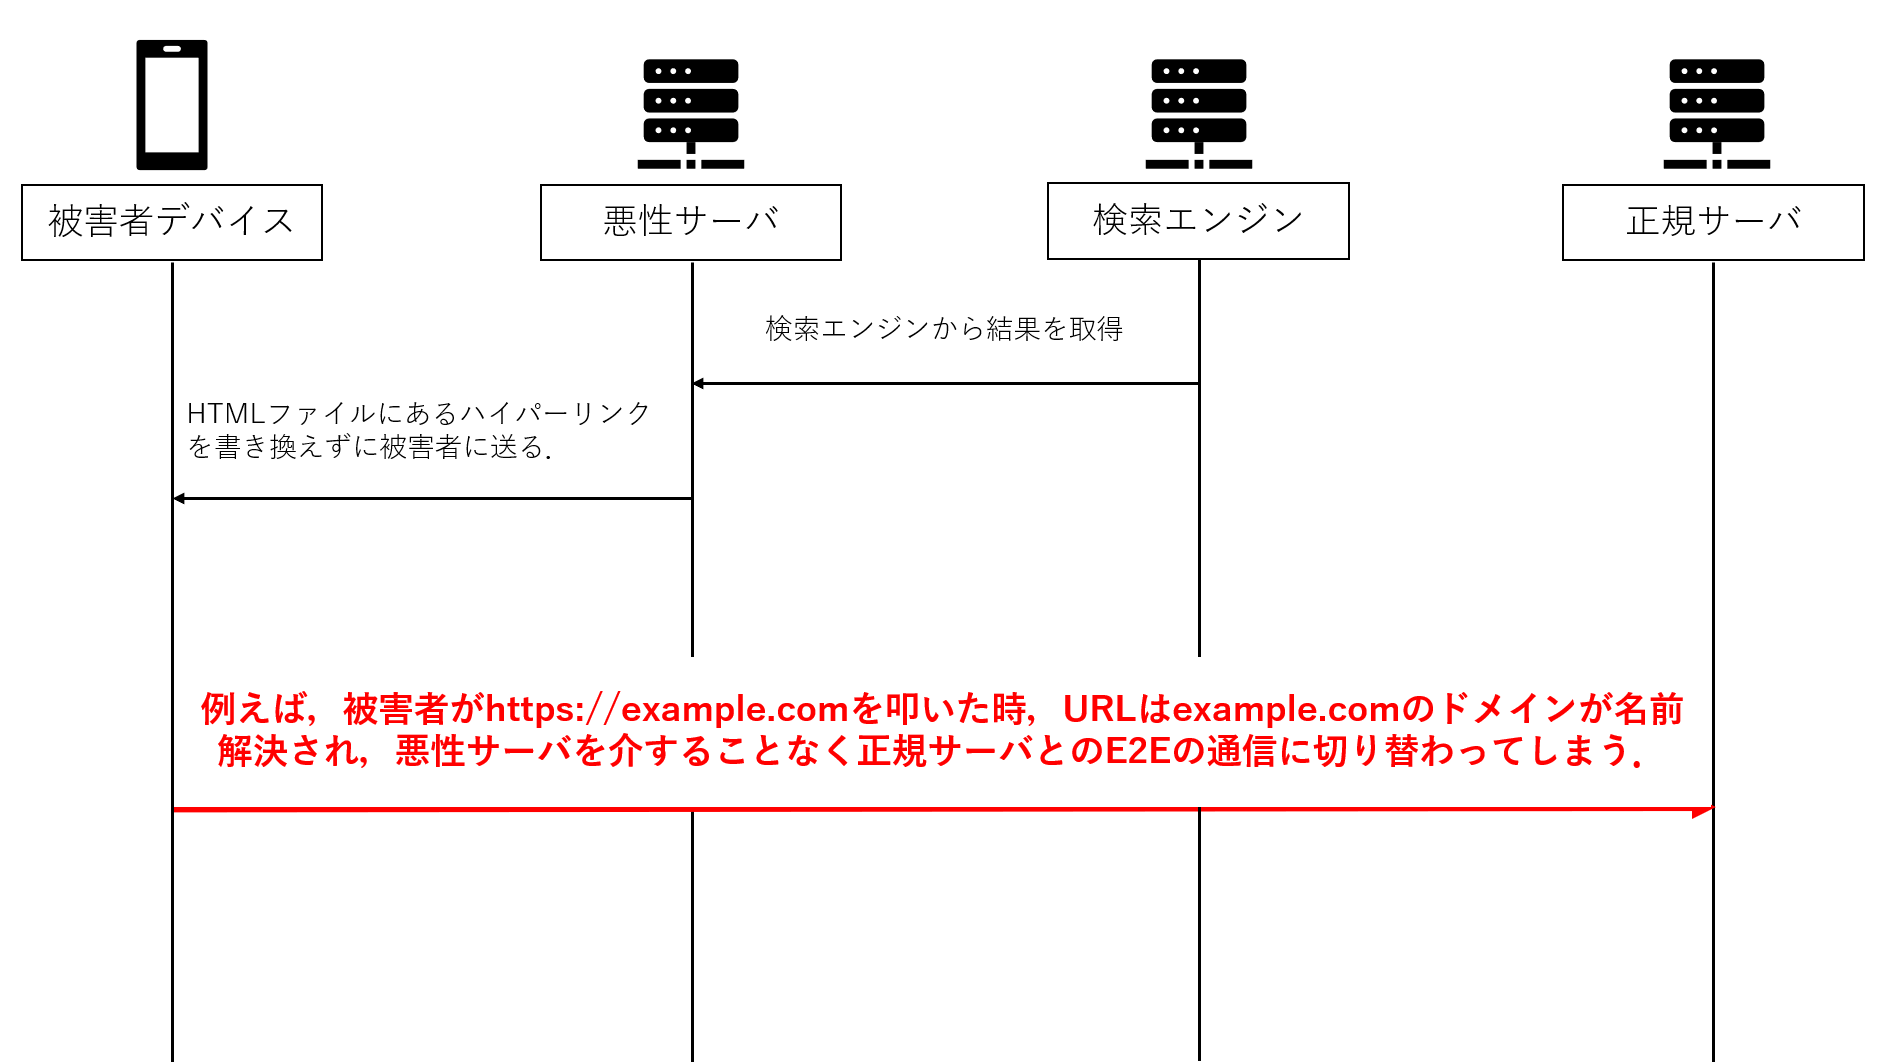
\includegraphics[width=12cm]{img/vc-vf-4-5-00.png}
                    \caption{HTMLファイル内のハイパーリンクを書き換えなかった場合の挙動}
                    \label{flow-no45-00}
                    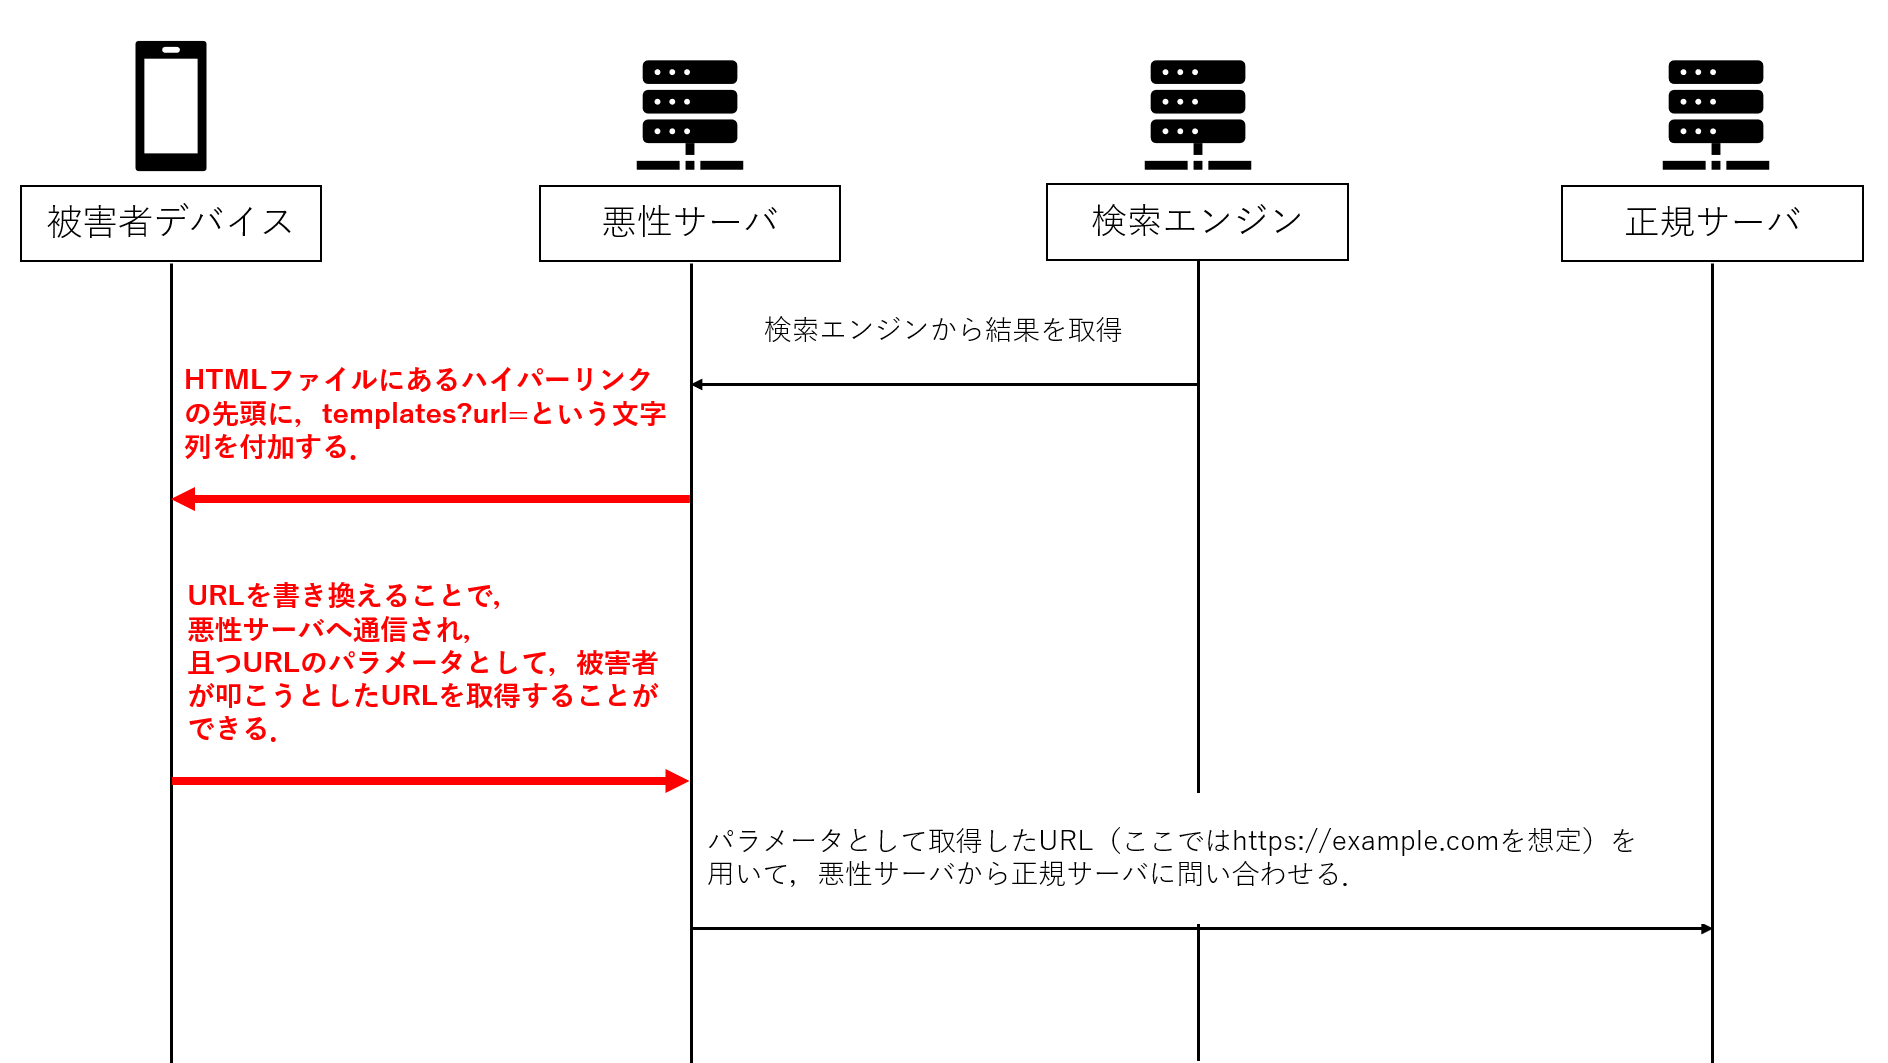
\includegraphics[width=12cm]{img/vc-vf-4-5-01.png}
                    \caption{HTMLファイル内のハイパーリンクを書き換えた場合の挙動}
                    \label{flow-no45-01}
                    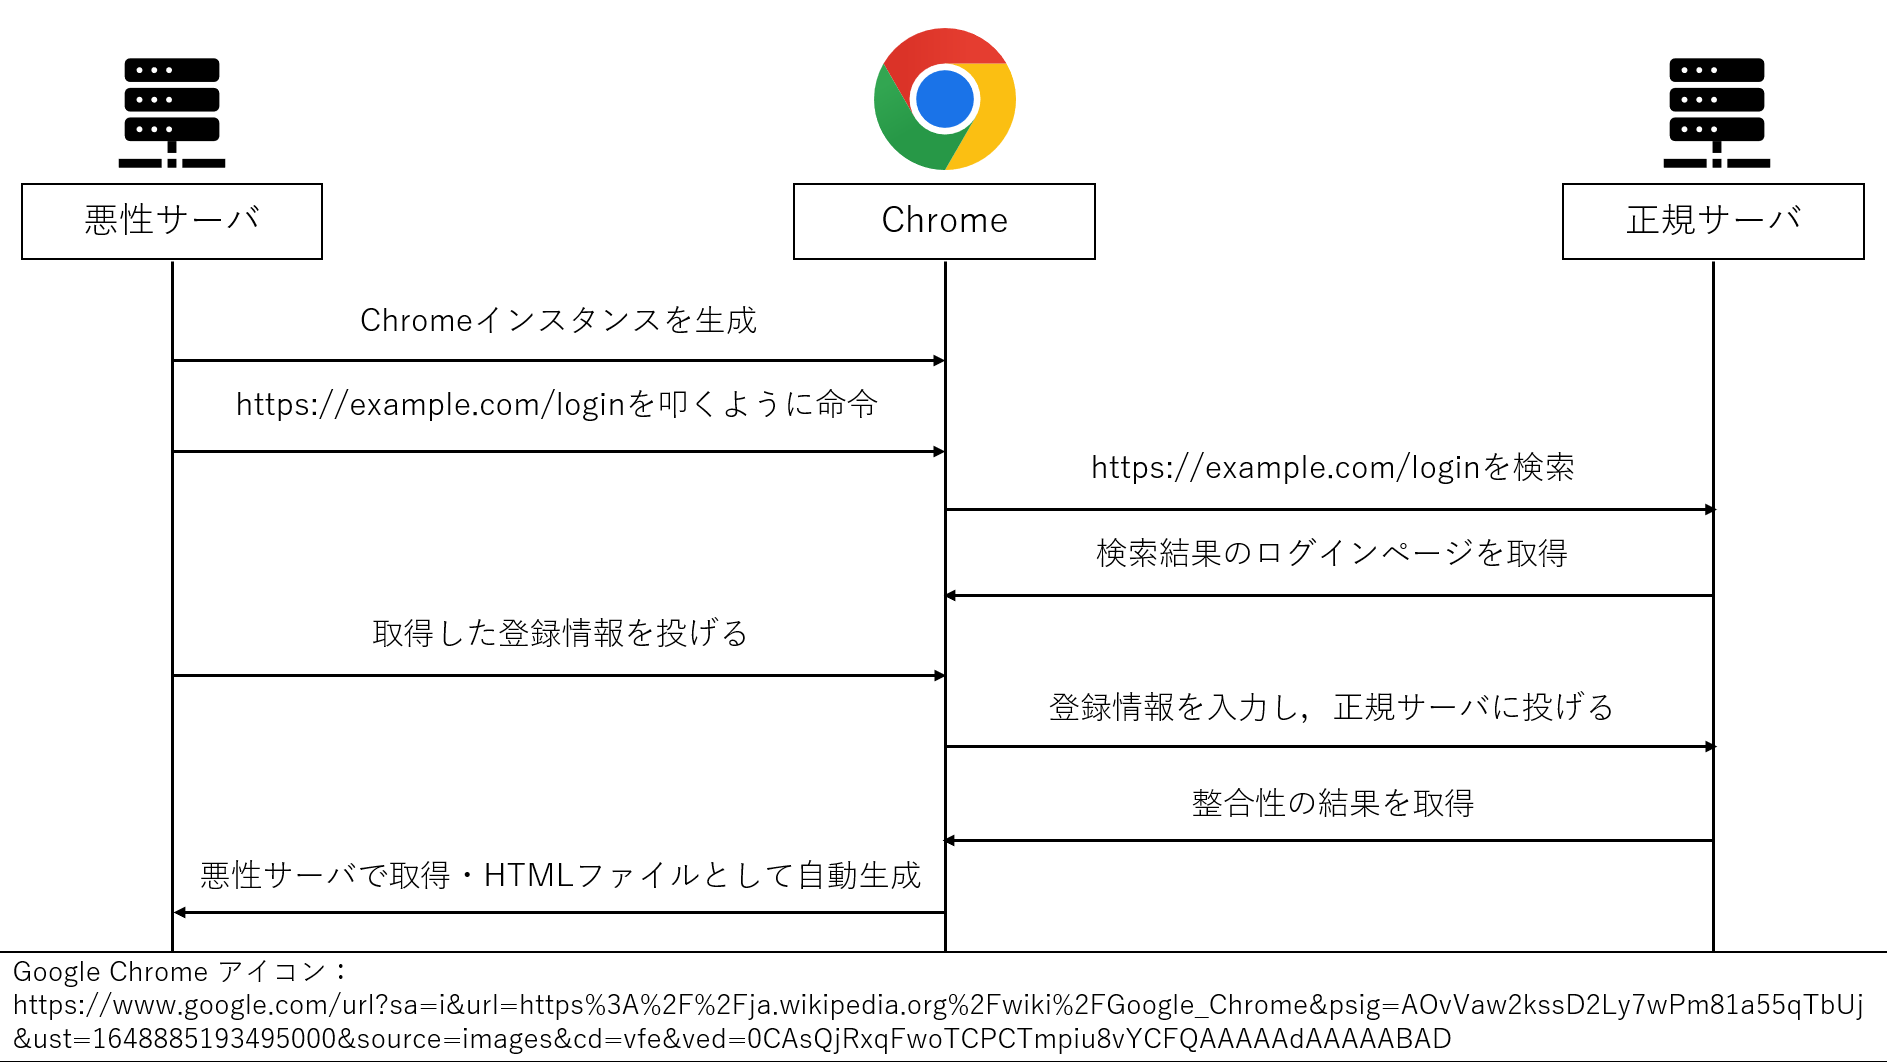
\includegraphics[width=12cm]{img/vc-vf-6-7.png}
                    \caption{登録情報の整合性の確認を行う流れ}
                    \label{flow-6-7}
                \end{figure*}
                \clearpage
    \section{システム評価}
        \subsection{楽天の場合}
            \subsubsection{動作結果}
                まず,認証画面への遷移し(図\ref{rakuten-00}),認証が終了すると偽の検索エンジンが表示される(図\ref{rakuten-01}).\
                ここの検索欄に「楽天通販」と検索して,その検索結果を待つ.\
                「楽天通販」と検索して得られた結果を表示する(図\ref{rakuten-02}).\
                ここで,被害者はGoogleの検索結果が得られたものと認識し,表示された楽天通販の結果から該当のサイトへのリンクをクリックする.\
                ここまでの動作は,図\ref{flow-no45-01}に準じて処理されたものである.\
                \begin{figure}[h]
                    \centering
                    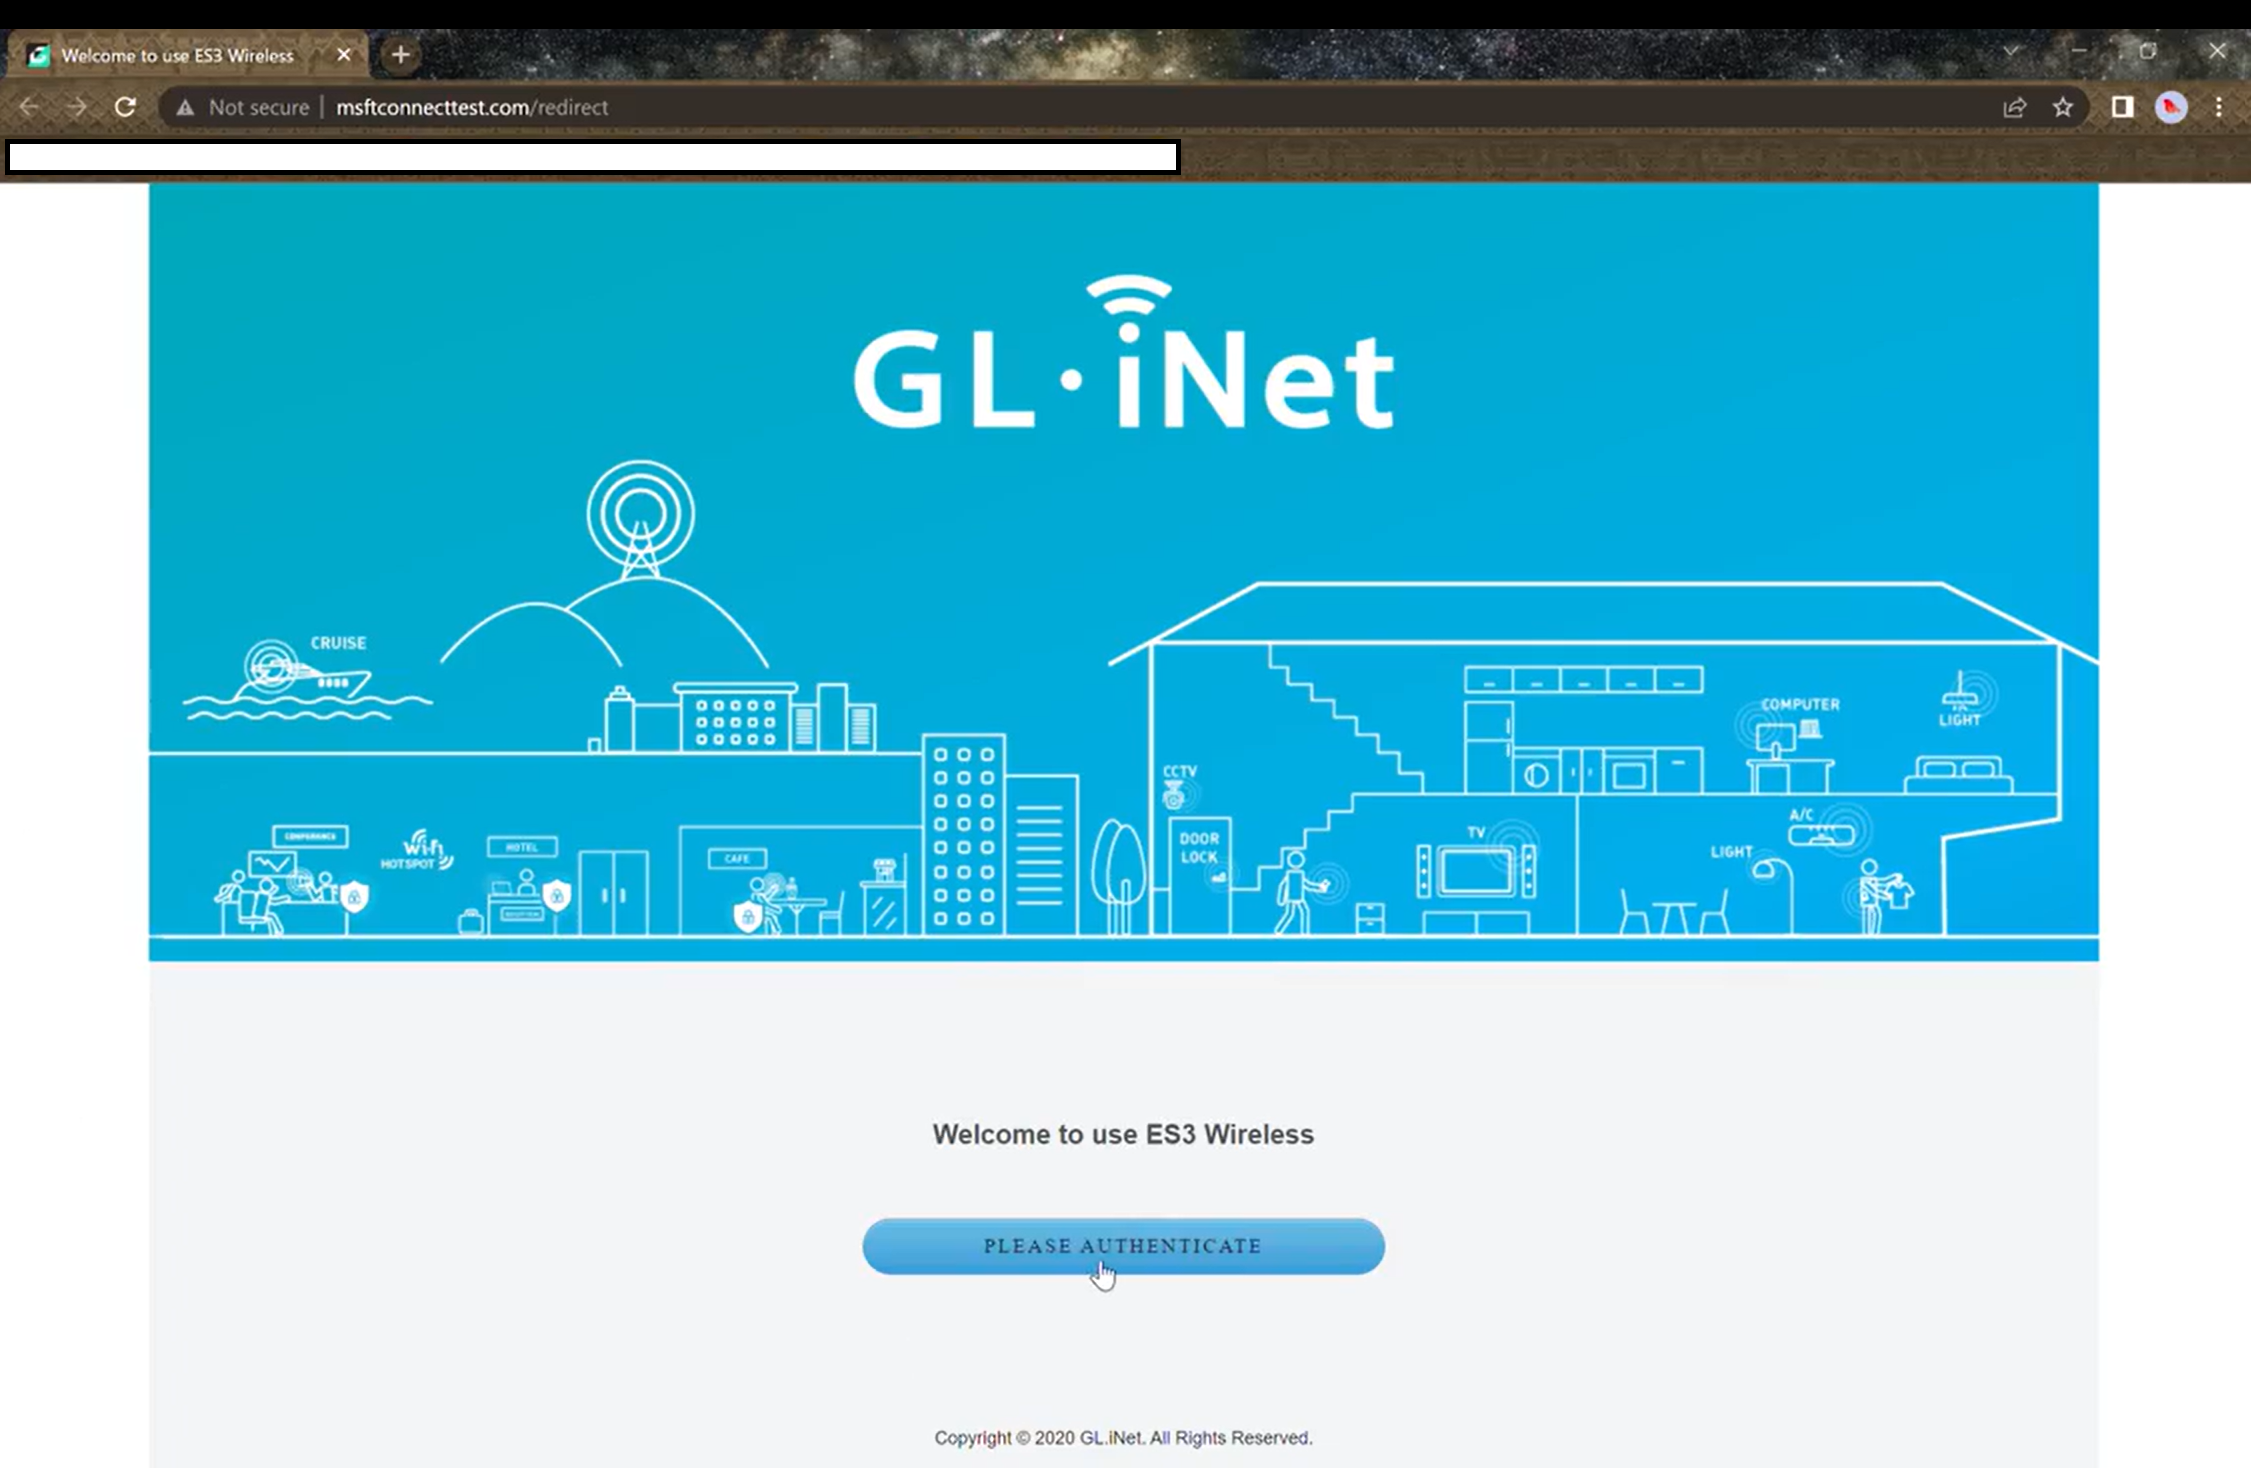
\includegraphics[width=6cm]{img/rakuten/rakuten-00.png}
                    \caption{認証画面}
                    \label{rakuten-00}
                    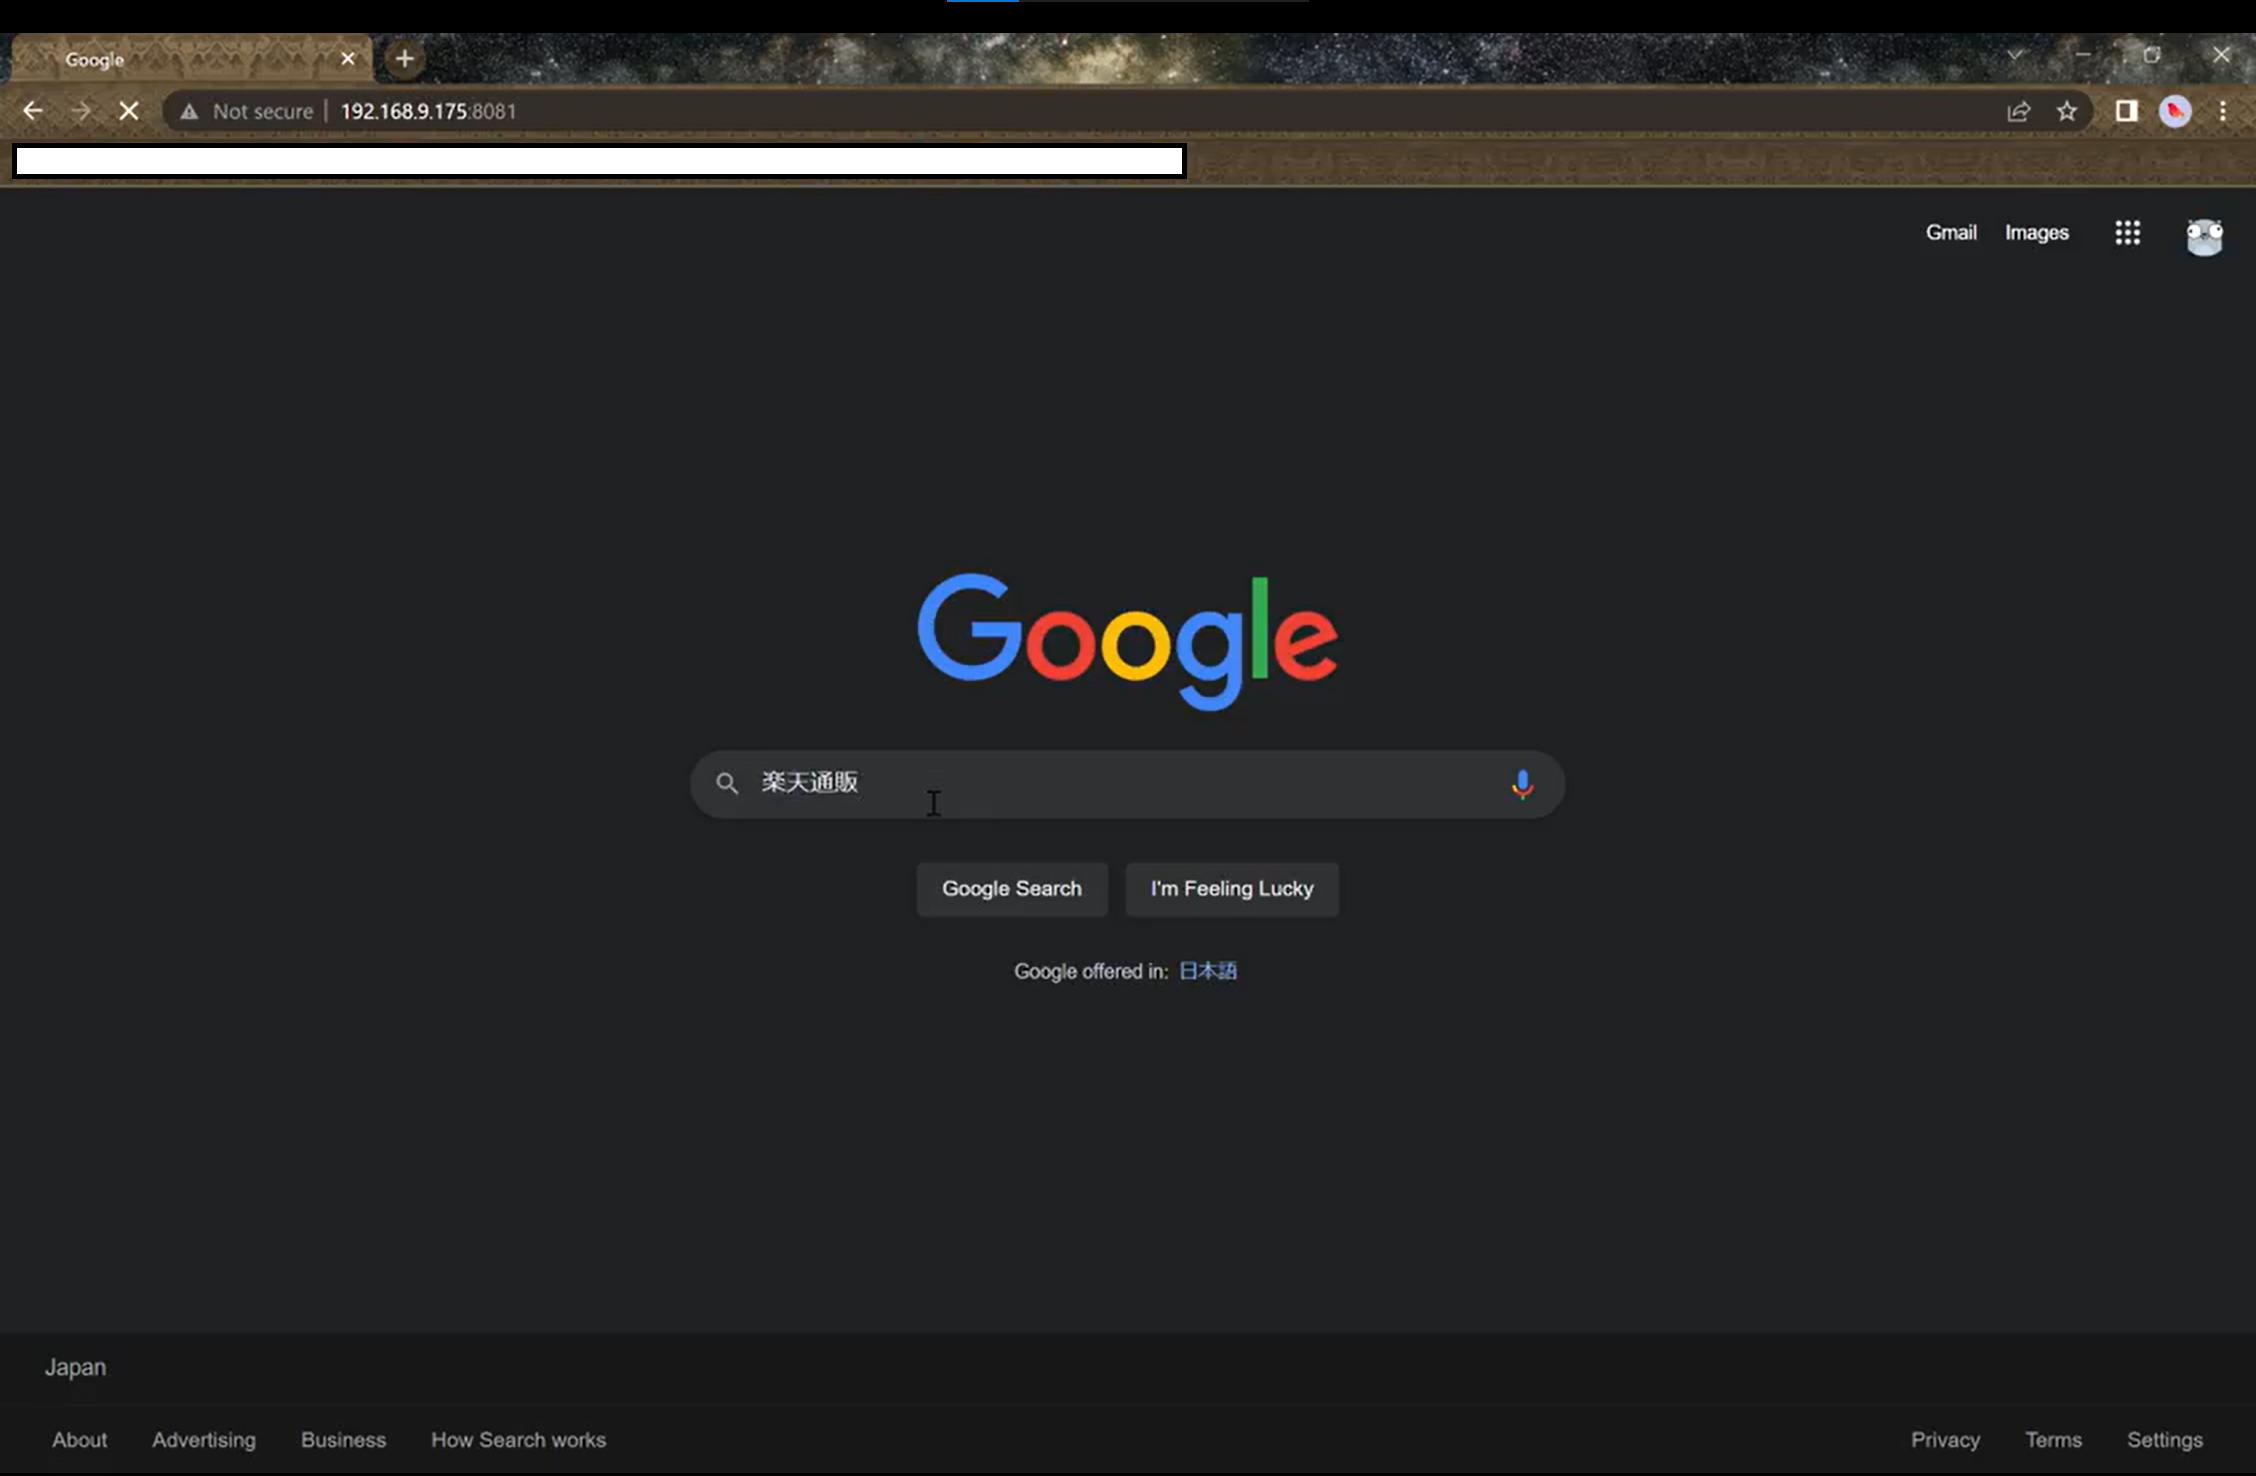
\includegraphics[width=6cm]{img/rakuten/rakuten-01.png}
                    \caption{偽のGoogle検索画面}
                    \label{rakuten-01}
                    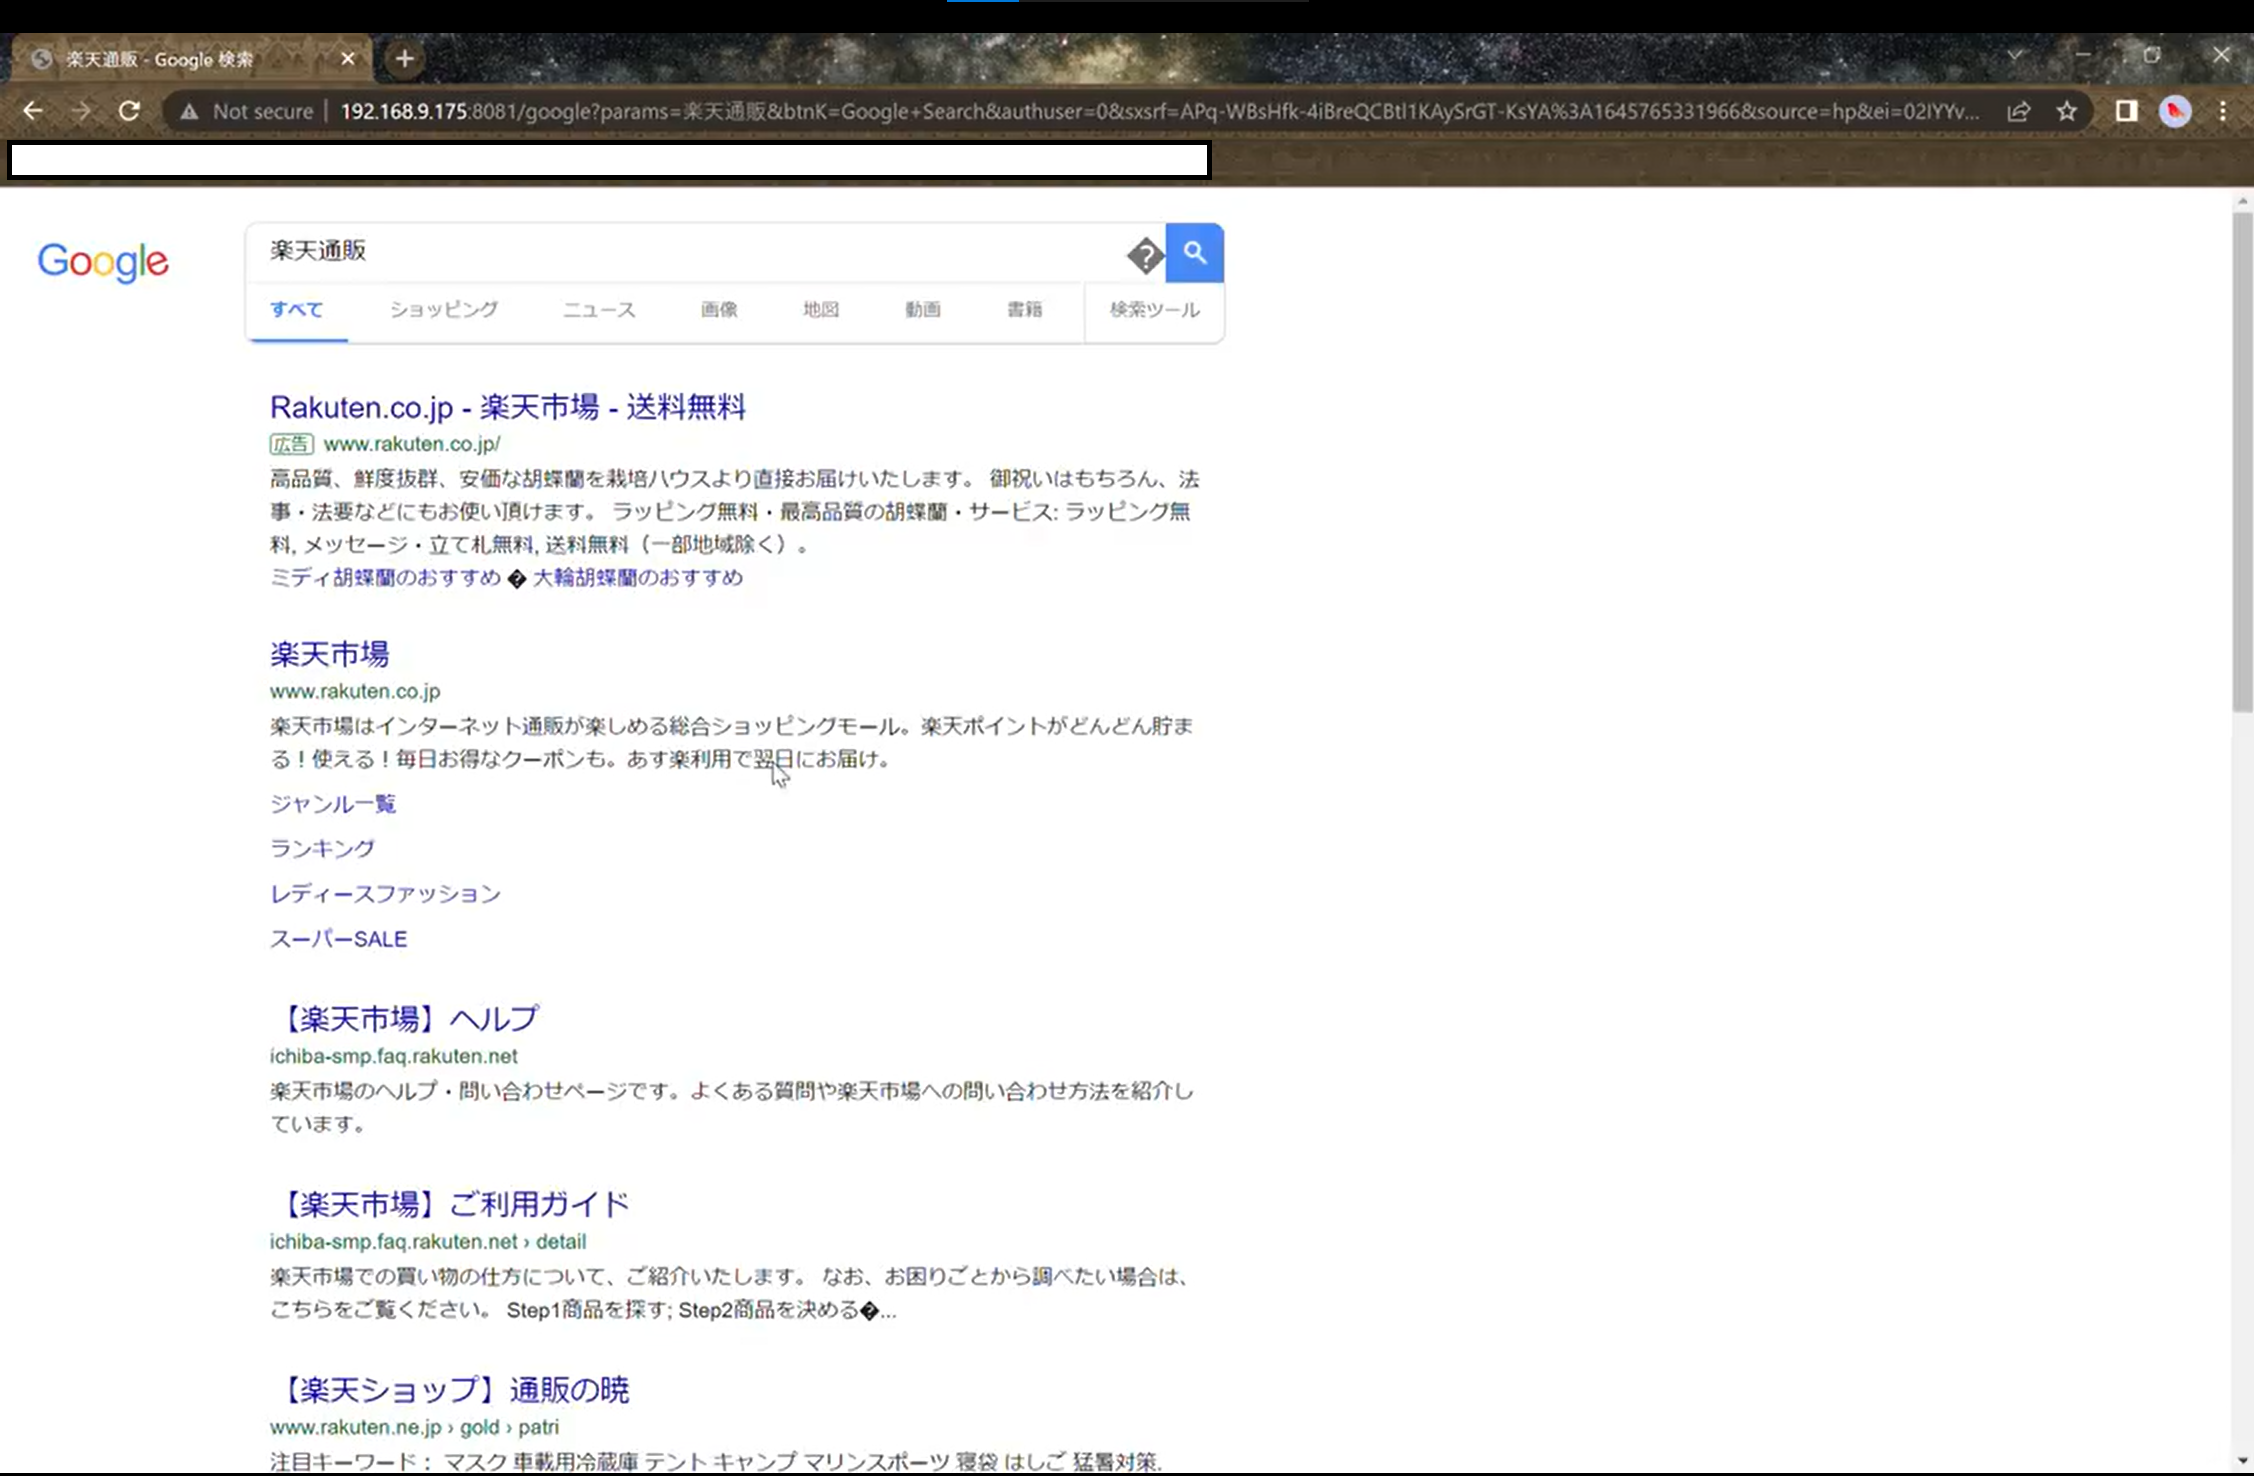
\includegraphics[width=6cm]{img/rakuten/rakuten-02.png}
                    \caption{「楽天通販」と検索した際の画面}
                    \label{rakuten-02}
                \end{figure}
                \\
                 得られて検索結果の画面から,楽天通販サイトに入る.\
                特に目立った文字化けや画像切れは起こっていない事から,ここまでも被害者は.楽天通販サイトに遷移したと認識する物とする.\
                ここで,個人アカウントに入る為に「ログイン」ボタンを押す(図\ref{rakuten-03}).\
                「ログイン」ボタンを押した結果は以下のようになる(図\ref{rakuten-04}).\
                このログイン画面は,攻撃が予め用意して攻撃者サーバにパラメータを送信させるように実装されたものである.\
                ここに,実際に自分のアカウント情報を入力し,「ログイン」ボタンを押す.\
                \begin{figure}[h]
                    \centering
                    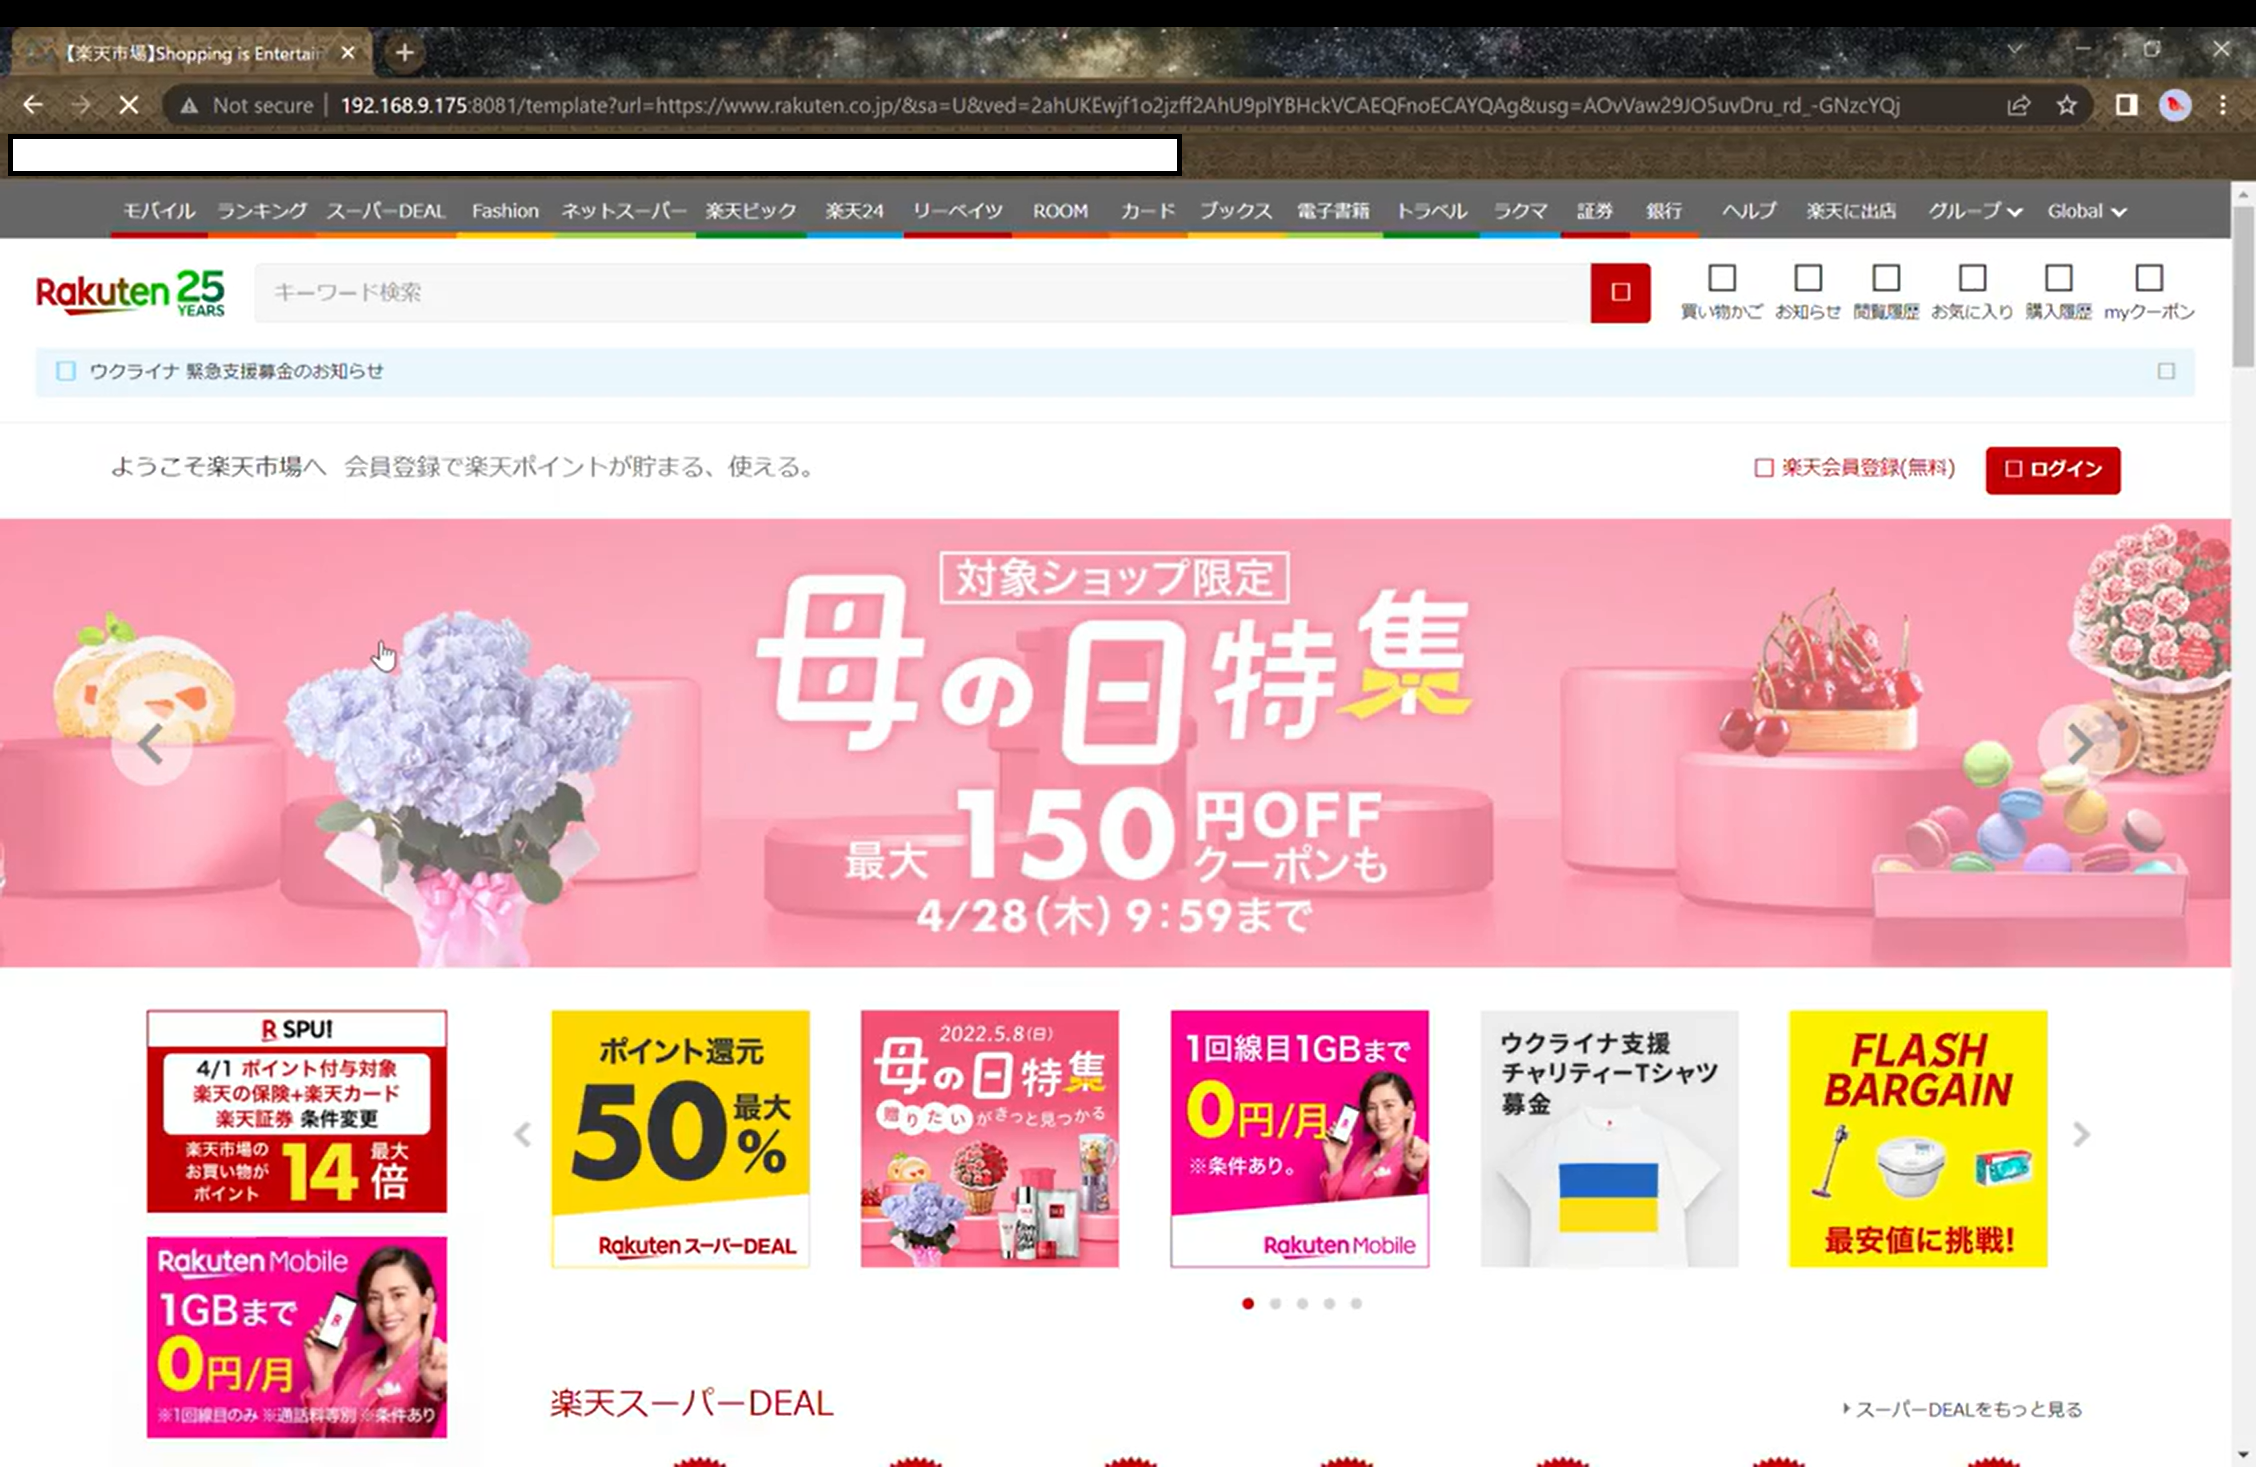
\includegraphics[width=6cm]{img/rakuten/rakuten-03.png}
                    \caption{検索結果の画面から楽天の複製サイトへ侵入した際の画面}
                    \label{rakuten-03}
                    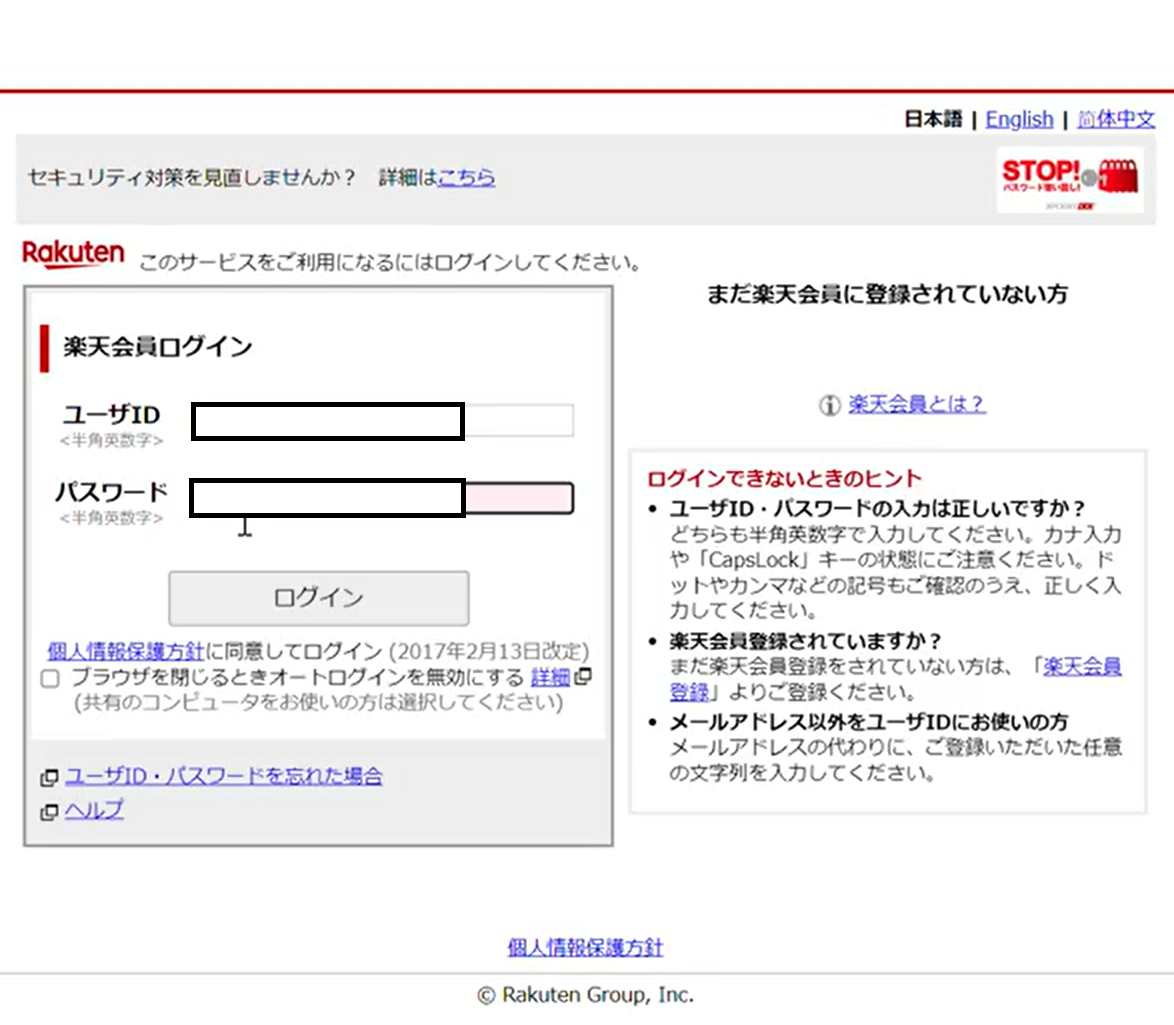
\includegraphics[width=6cm]{img/rakuten/rakuten-04.png}
                    \caption{ログイン画面へ入り,登録情報を入力した際の画面}
                    \label{rakuten-04}
                \end{figure}
                \\
                 入力されたパラメータを攻撃者サーバ内から処理をし,正規サーバから返却された結果を被害者に提示する.\
                図\ref{rakuten-05}は,実際に個人アカウントに侵入した結果である.\
                ここまでの動作は図\ref{flow-6-7}に準じて処理されており,目立った警告や画像切れ無く且つ正規サーバとの通信を中継する形で個人アカウントへのログインに成功した.\
                \begin{figure}[h]
                    \centering
                    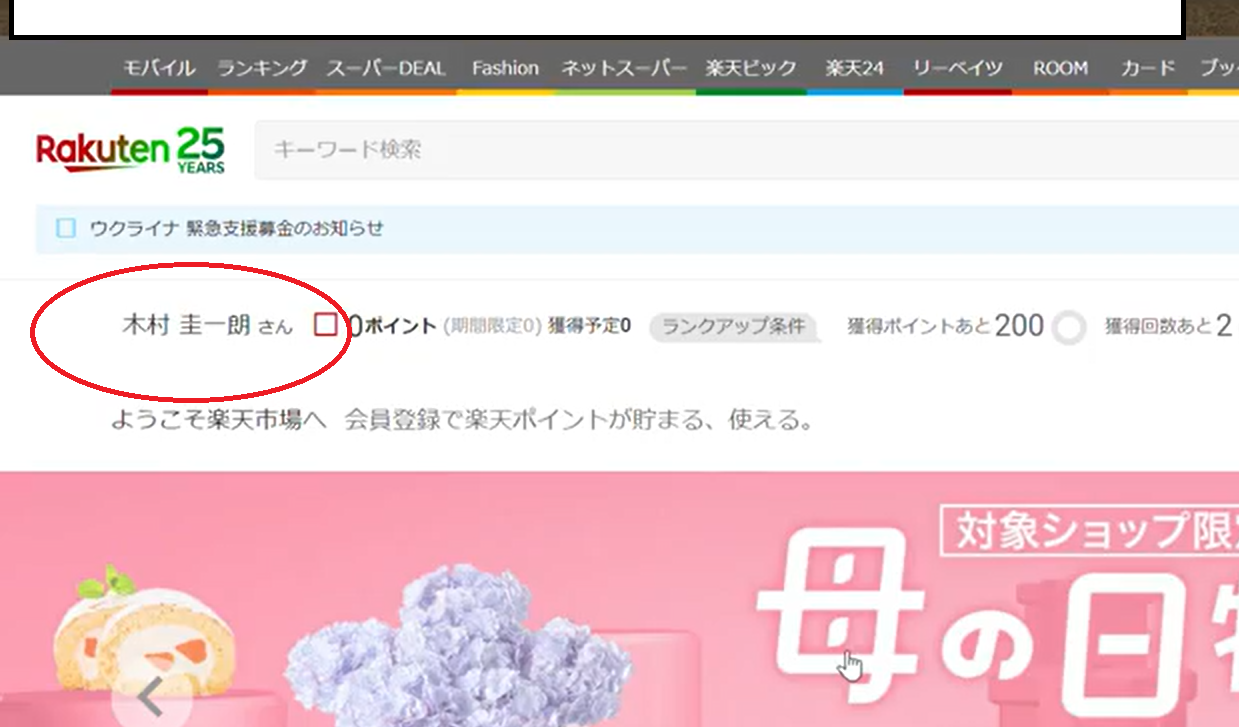
\includegraphics[width=6cm]{img/rakuten/rakuten-05.png}
                    \caption{ログイン情報の整合が取れ,実際に個人アカウントへログインした後の画面}
                    \label{rakuten-05}
                \end{figure}
            \subsubsection{問題点}
                楽天の場合の主な問題点として,ログイン情報の入力から実際にログインが完了されるまで,ある程度の時間を要する事が挙げられる.\
                具体的な実行時間の結果を\ref{calc-run-time}に示す.\
                \begin{table}[h]
                    \centering
                    \caption{Amazonと楽天の実行時間比較}
                    \begin{tabular}{lll}
                    \hline
                        & 楽天           & Amazon      \\ \hline
                    1回目  & 24.73{[}s{]} & 6.64{[}s{]} \\
                    2回目  & 24.65{[}s{]} & 6.98{[}s{]} \\
                    3回目  & 24.43{[}s{]} & 7.30{[}s{]} \\
                    4回目  & 24.81{[}s{]} & 7.35{[}s{]} \\
                    5回目  & 24.43{[}s{]} & 7.27{[}s{]} \\
                    6回目  & 24.86{[}s{]} & 7.55{[}s{]} \\
                    7回目  & 24.37{[}s{]} & 7.51{[}s{]} \\
                    8回目  & 25.43{[}s{]} & 7.45{[}s{]} \\
                    9回目  & 24.38{[}s{]} & 7.63{[}s{]} \\
                    10回目 & 24.61{[}s{]} & 7.31{[}s{]} \\ \hline
                    \end{tabular}
                    \label{calc-run-time}
                \end{table}
                \\
                この原因は,主に二つ考えられる.\
                一つ目は,ログインのプロセスに複数の処理が絡んでいる点にある.\
                具体なプロセスは,図\ref{flow-6-7}に示すプロセスに加え,結果の出力と悪性サーバに通信するようにするためのURLの書き換えプロセスの含まれいてる.\
                しかし,書き換えプロセスにはさほど実行時間を要さない為,実行時間の長さはChromedpの一連の処理による部分が大きいと考えられる.\
                二つ目は,Chromedpからログイン結果を取得しようとした場合,最低でも13秒程度待機しなければ,ログイン後の画面のHTMLを確実に取得できない点にある.\
                これは,実装段階で待機秒数を決定する時に判明した.\
                今回はログイン後の画面を確実に取得する為に,デフォルトで13秒待機を設定している為,実行時間が必然的に長くなってしまっている.\
        \subsection{Amazonの場合}
            \subsubsection{動作結果}
                まず,図\ref{rakuten-00}と同様に悪性のAPにアクセスし,認証を終了させた後,図\ref{rakuten-01}のように偽のGoogle検索エンジンが表示され,Amazon通販と入力して検索結果を取得し(図\ref{amazon-00}),そこから複製されたAmazonの通販サイトに遷移した.\
                続いて,ログインを行う為に画面右上にあるログインボタンを押して個人アカウントへの侵入に試みた(図\ref{amazon-01}).\
                \begin{figure}[h]
                    \centering
                    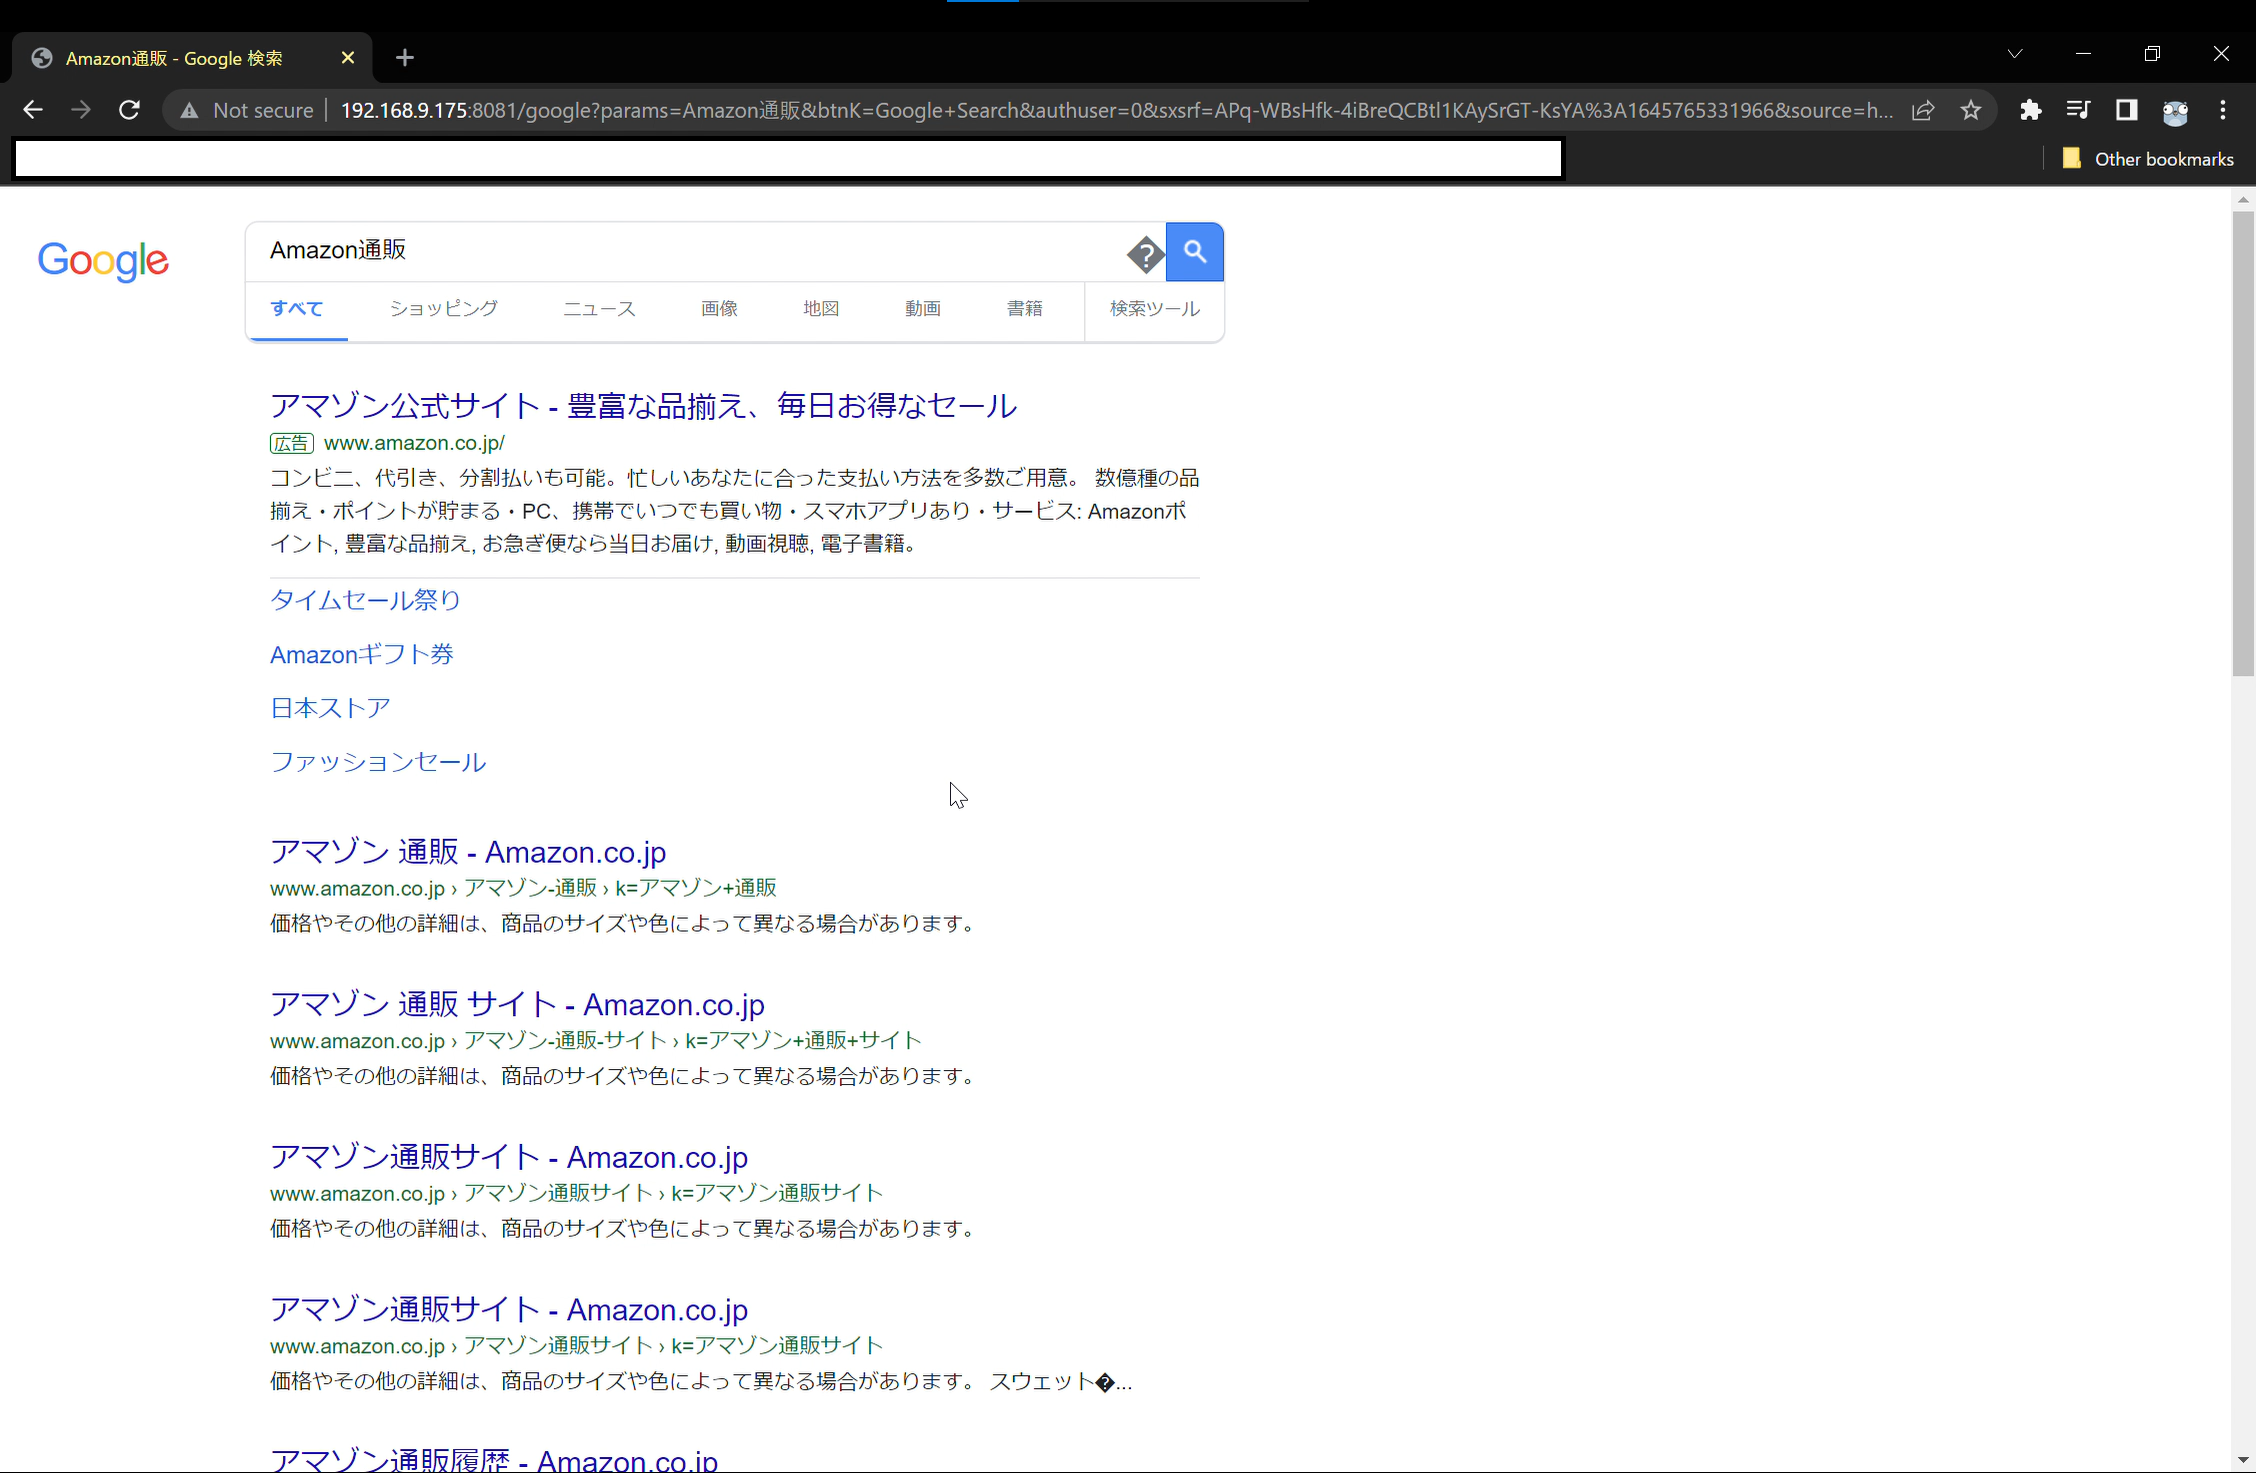
\includegraphics[width=6cm]{img/amazon/amazon-00.png}
                    \caption{「Amazon通販」と検索した際の画面}
                    \label{amazon-00}
                    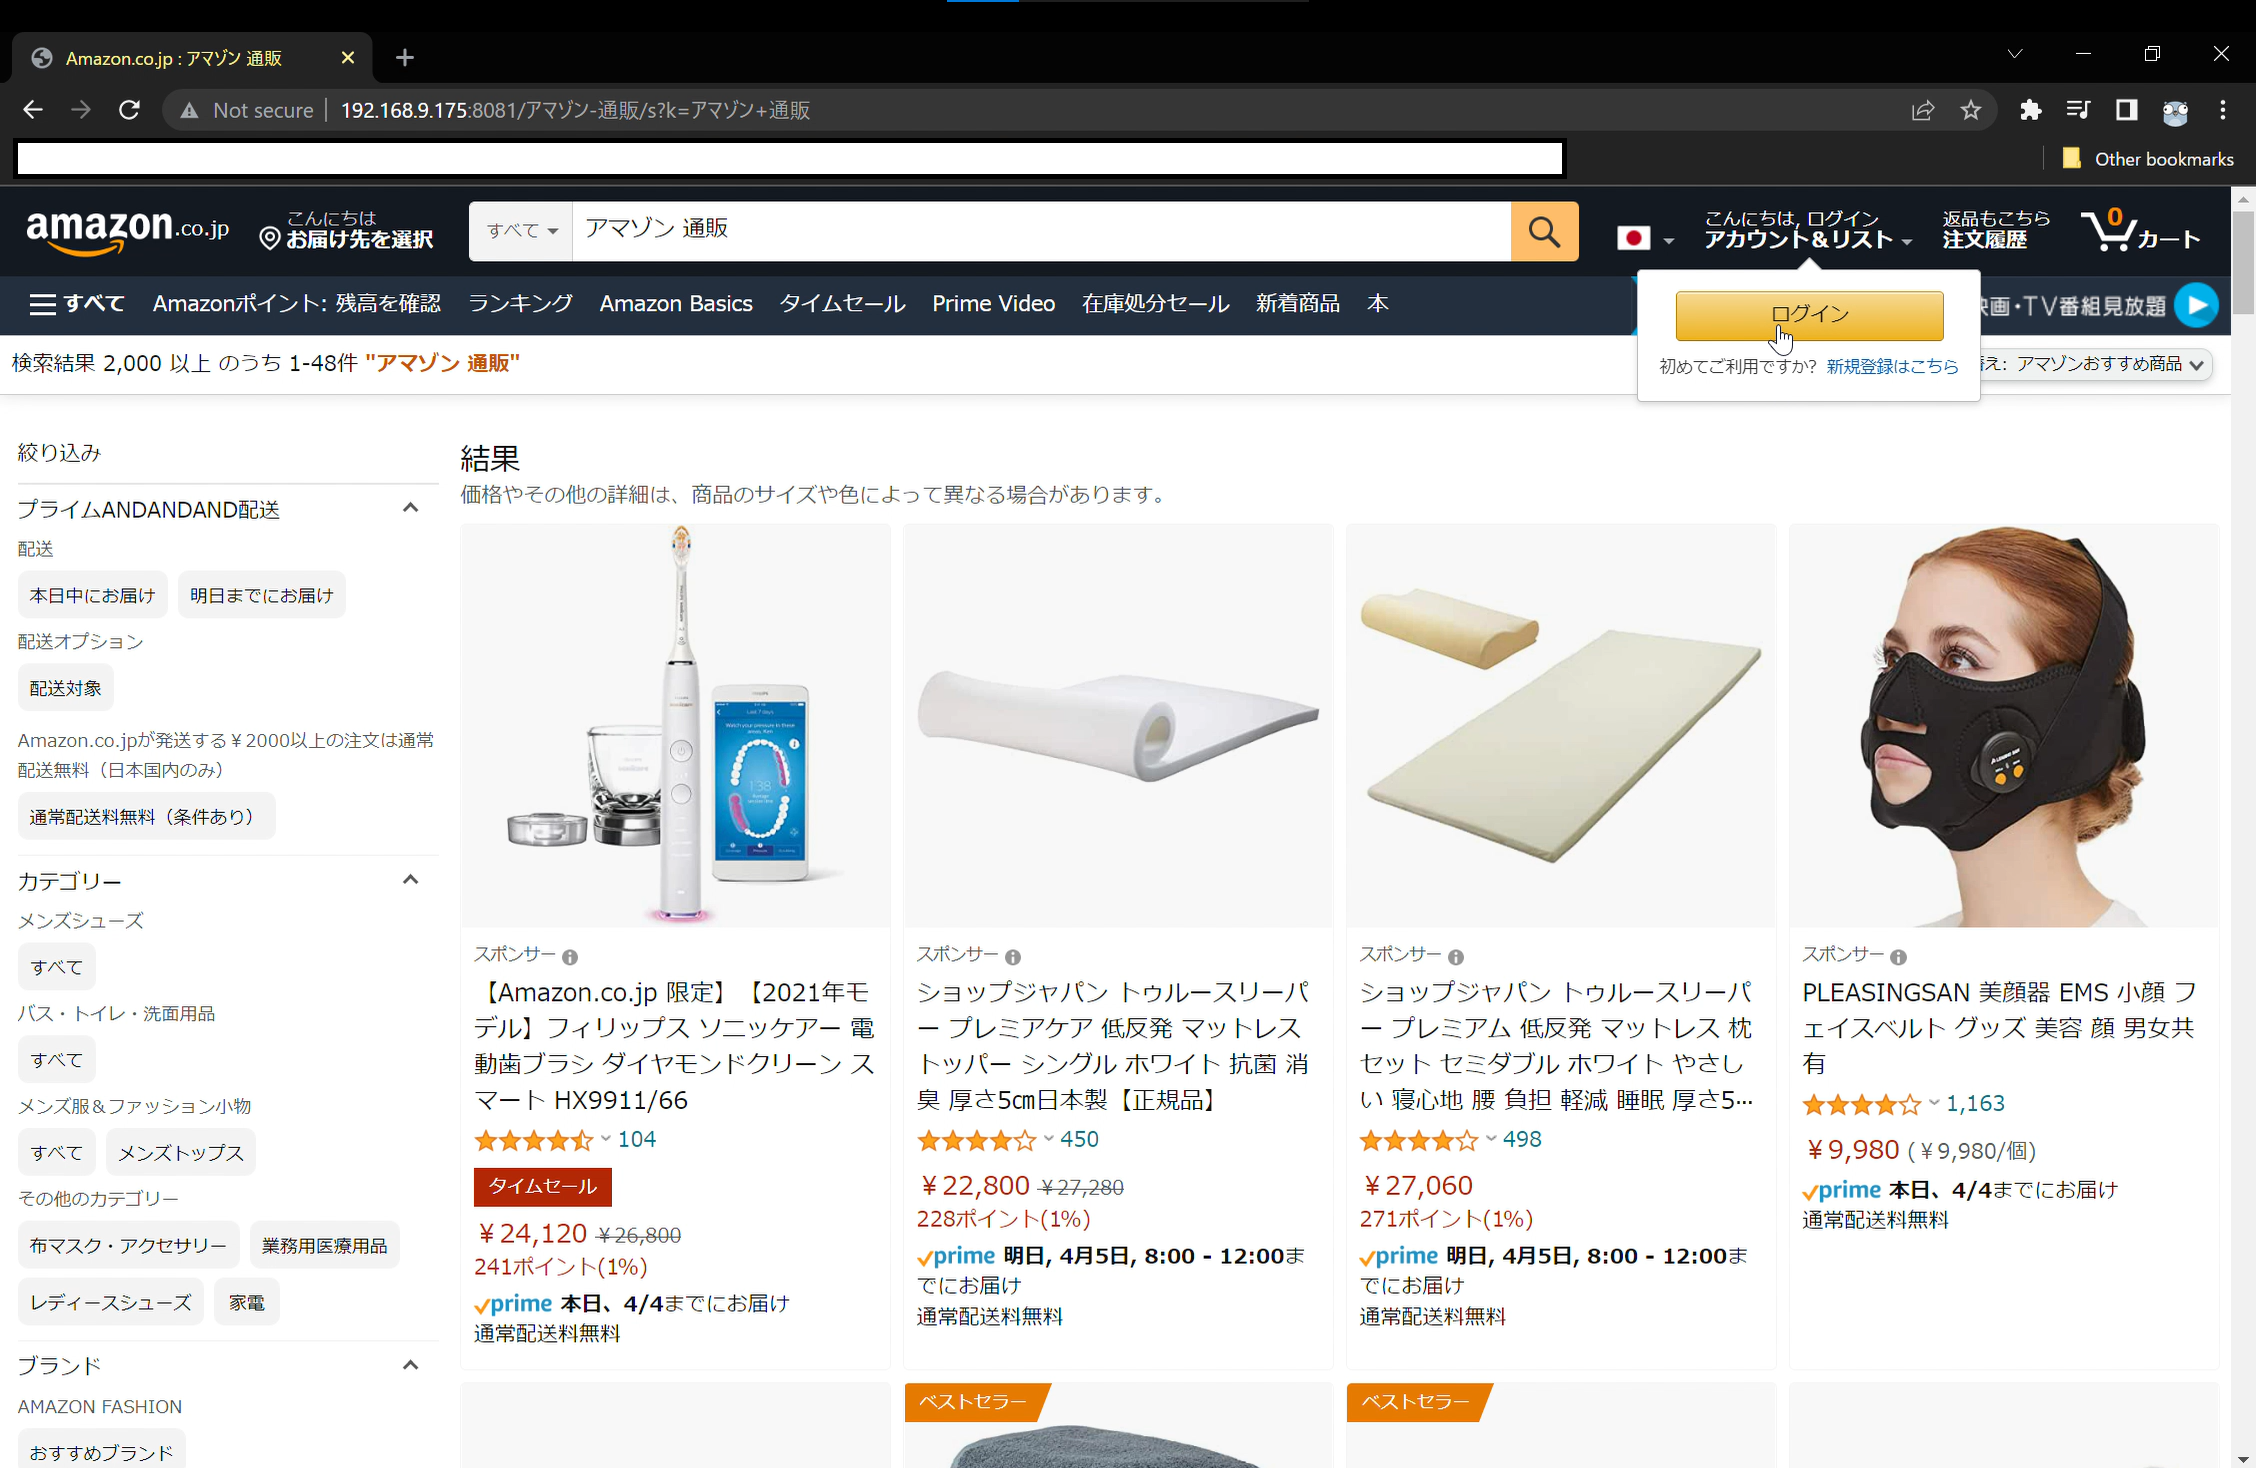
\includegraphics[width=6cm]{img/amazon/amazon-01.png}
                    \caption{検索結果の画面からAmazonの複製サイトへ遷移した際の画面}
                    \label{amazon-01}
                \end{figure}
                \\
                ログインボタンを押すと,ログイン画面に遷移した(図\ref{amazon-02}).\
                この画面は予め攻撃者側で作成したもので.入力フォームとその入力データの送信を悪性サーバ側で取得するようにしている.\
                この入力フォームに,実際にアカウント情報を入力してログインボタンを押した.\
                入力情報をサーバ側で取得して,図\ref{flow-6-7}の手順に従い入力情報の処理を行った.\
                そして,入力情報の整合性の確認が完了し,実際に個人アカウントへの侵入に成功した.\
                図\ref{amazon-03}の右上には,実際に個人アカウントの名前が明記されていることが分かる.\
                ここまでの動作は図\ref{flow-6-7}の動作に従って処理されており,楽天と同様に目立った画像切れや警告を出さずに,且つ正規サーバとの通信を攻撃者が中継する形で個人アカウントに侵入することができた.\
                \begin{figure}[h]
                    \centering
                    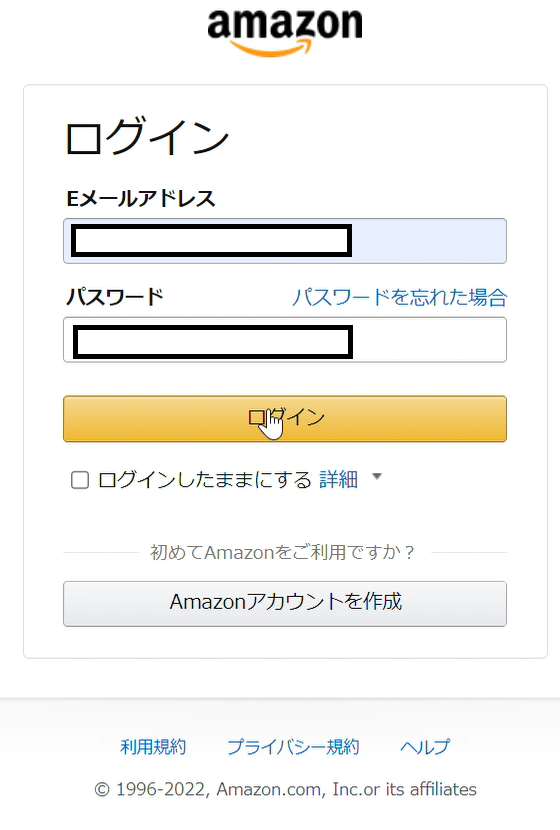
\includegraphics[width=6cm]{img/amazon/amazon-02.png}
                    \caption{ログイン画面へ入り,登録情報を入力した際の画面}
                    \label{amazon-02}
                    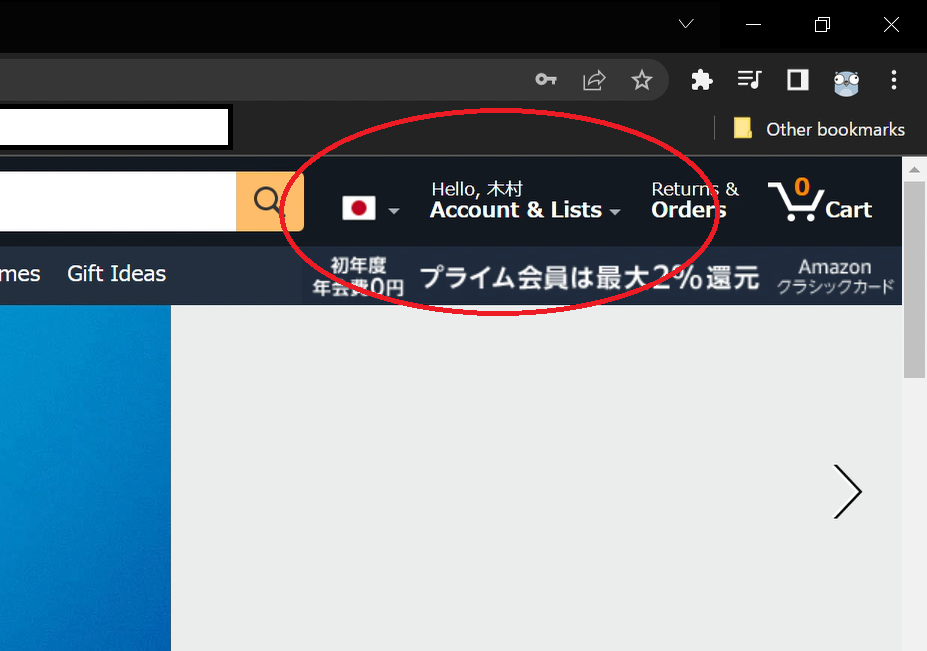
\includegraphics[width=6cm]{img/amazon/amazon-03.png}
                    \caption{ログイン情報の整合が取れ,実際に個人アカウントへログインした後の画面}
                    \label{amazon-03}
                \end{figure}
            \subsubsection{問題点}
                Amazonの場合,場合によればCAPTCHAに引っかかりログイン画面を突破できない場合があるという問題点が挙げられる.\
                CAPTCHAとは,自動化されたボットによるWebサイトの操作を防止するもので,例えば,人間は認識可能でボットには認識不可能な歪みを含んだ文字列を提示し,その文字列を入力させる事で人間かボットかを認識するようなものが挙げられる(図\ref{captcha}).\
                今回の実装では,CAPTCHAを回避或いはCAPTCHAの文字列を被害者に入力させて突破させる事はできなかった.\
                \begin{figure}[h]
                    \centering
                    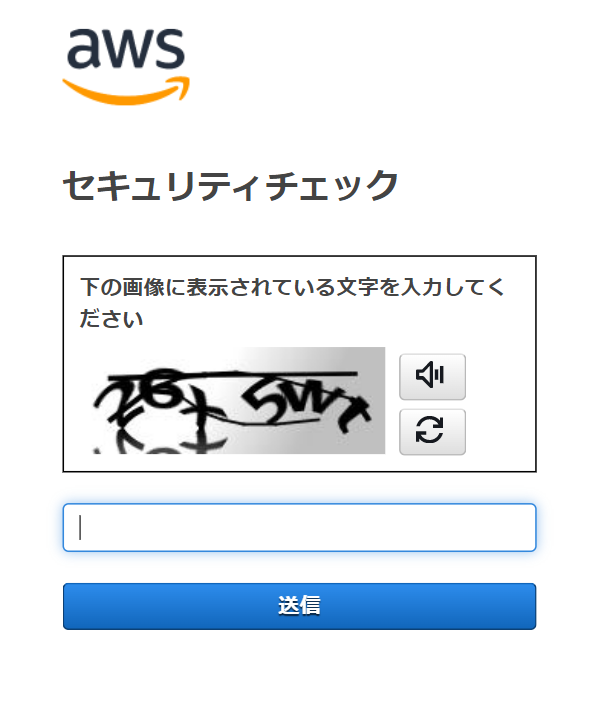
\includegraphics[width=6cm]{img/captcha.png}
                    \caption{CAPTCHAの例:AWSコンソールにログインする際に実際に出るCAPTCHAの一例}
                    \label{captcha}
                \end{figure}
        \subsection{評価}
            今回,「楽天」と「Amazon」の二つの通販サイトに絞ってシステムの構築を行ったが,両者ともブラウザ上での警告を出さずに個人情報の傍受・窃取が可能であることが分かった.\
            加えて,被害者のブラウザに対しても明確な警告の表示や画像切れが見れなかった為,通信の中継としての役割を十分に担う事ができていると評価できる.\\
             しかし,いくつかの問題点も残されている.\
            前節の検証結果でも述べたものを改めて列挙すると,次のようになる.\
            \begin{enumerate}
                \item (楽天の場合)登録情報の整合性の確認にやや時間を要する点.
                \item (Amazonの場合)CAPTCHAに引っかかり,ログインできない場合がある点.
            \end{enumerate}
             まず1についてであるが,これは6.1.2問題点にも記述したように,Chromedpを利用して個人情報の整合性の確認を行う際に非常に時間を要している点が主な原因と考えられる.\
            具体的な処理プロセスは,(1)Chromeインスタンスの作成,(2)ブラウザを開き楽天のログイン画面へ遷移,(3)指定のJS Pathを検索し個人情報を入力,(4)ログイン,(5)得られた結果をHTMLとして抽出,の計5行程となってるが.ログイン後の結果を完全に取得しようとした際,(4)と(5)の行程で約13秒程度待機する必要がある点が主なボトルネックとなっている.\
            今後の課題としては,Chromedpに依存していない部分の実行時間の削減に加え,今回の処理が別の言語で実行できる場合,Golangの場合との実行時間の比較を行い,ボトルネックの解消の可能性を探る必要がある.\\
             続いて,2についてであるが,CAPTCHAに引っかかる主な原因は,個人情報をプログラムで入力している点が原因である.\
            ブラウザ情報を維持したChromeインスタンスをCAPTCHAの回避を目的として再度別の処理で再利用する場合,Chromeインスタンスのリロードが必要となる.\
            しかし,Chromeインスタンスのリロードはブラウザ画面のリロードと同様の挙動を示すため,その際にCHATCHAとして表示された文字列も変わってしまう.\
            従って,被害者がCAPTCHAの文字列を入力したとしても,結果的に整合性が取れない.\
            現在,このCAPTCHAの問題を解決する具体的な実装はできていない為,今後も回避方法を考えていく必要がある.\
    
    \section{あとがき}
        本稿では,Captive Portalの認証後に飛ばされるサイトを起点として,クライアントとサーバ間の通信に攻撃者を中継させ,通信内容及び機密情報の傍受・窃取を行う手法について提案し,ターゲットを絞った実証を通し,その有効性を確認した.\
        この手法では,クライアントはセッションフェーズからサーバと直接やり取りをすることはない為,サーバ側がSSL/TLS通信を強制するものに関係なく通信の傍受・窃取を行う事が可能である.\
        今後は,ターゲットを更に拡張,或いは汎用性のある実装へのリファクタリングを行う事で,機密情報を扱う幅広いサイトに対して通信内容の傍受・窃取を可能にすることを課題とし,改良を重ねていく.

    \section{参考文献}
        \begin{thebibliography}{9}
            \bibitem{SoumuWiFi} 総務省,2020年に向け全国約3万箇所のWi-Fi整備を目指して,\url{https://www.soumu.go.jp/main_content/000548781.pdf}
            \bibitem{IPA} IPA,公衆無線LAN利用に係る脅威と対策 ~公衆無線LANを安全に利用するために~,\url{https://www.ipa.go.jp/files/000051453.pdf}
            \bibitem{FakeAP} \textit{LUNODZO J. MWINUKA, ABEL Z. AGGHEY, SHUBI F. KAIJAGE, (Senior Member, IEEE), AND JEMA D. NDIBWILE: FakeAP Detector: An Android-Based Client-Side Application for Detecting Wi-Fi Hotspot Spoofing}
            \bibitem{ETGuard} \textit{Vineeta Jaina, Vijay Laxmi, Manoj Singh Gaur, Mohamed Mosbah: ETGuard: Detecting D2D attacks using wireless Evil Twins}
            \bibitem{SslStrip} \textit{Moxie Marlinespike: New Tricks For Defeating SSL In Practice}
            \bibitem{HSTS} \textit{Takashi Setozaki, Kazuto Matsuo: An Enhanced Sslstrip Attack aginst HTTPS with HSTS}
            \bibitem{FakeSslAndDnsServer} \textit{MATSUMOTO Hiroaki(Tokei University), KODAMA Yosuke(Data Management), KIKUCHI Hiroaki(Meiji University), ISHII Hiroshi(Tokai University): On the risk of SSL Man-in-the-Middle Attack with dynamic fake SSL server certificates and DNS servers}
        \end{thebibliography}
        
    \section{付録}
        \subsection{実装コード}
            実装コードのGitHubリポジトリ \url{https://github.com/ES3-Kobe-U/go-malproxy}
        \subsection{Chromedp}
            ChromedpのGitHUbリポジトリ \url{https://github.com/chromedp/chromedp}
\end{document}